\documentclass[10pt,a4paper]{article}
\usepackage[latin1]{inputenc}
\usepackage{csquotes}
\usepackage[english]{babel}
\usepackage{amsmath}
\usepackage{amsfonts}
\usepackage{amssymb}
\usepackage{blkarray}
\usepackage{graphicx}
\usepackage{caption}
\usepackage{subcaption}
\usepackage{appendix}
\usepackage{listings}
\usepackage{xspace}
\usepackage{biblatex}
\usepackage{hyperref}
\bibliography{refs.bib}
\usepackage{color}
\definecolor{dkgreen}{rgb}{0,0.6,0}
\definecolor{gray}{rgb}{0.5,0.5,0.5}
\definecolor{mauve}{rgb}{0.58,0,0.82}

\newenvironment{changemargin}[3]{%
\begin{list}{}{%
\setlength{\topsep}{0pt}%
\setlength{\leftmargin}{#1}%
\setlength{\rightmargin}{#1}%
\addtolength{\topmargin}{#2}
\addtolength{\textheight}{#3}
\setlength{\listparindent}{\parindent}%
\setlength{\itemindent}{\parindent}%
\setlength{\parsep}{\parskip}%
}%
\item[]}{\end{list}}

\lstset{ %
  language=Octave,                % the language of the code
  basicstyle=\footnotesize,           % the size of the fonts that are used for the code
  numbers=left,                   % where to put the line-numbers
  numberstyle=\tiny\color{gray},  % the style that is used for the line-numbers
  stepnumber=1,                   % the step between two line-numbers. If it's 1, each line 
                                  % will be numbered
  numbersep=5pt,                  % how far the line-numbers are from the code
  frame=single,                   % adds a frame around the code
  rulecolor=\color{black},        % if not set, the frame-color may be changed on line-breaks within not-black text (e.g. commens (green here))
  tabsize=8,                      % sets default tabsize to 2 spaces
  captionpos=b,                   % sets the caption-position to bottom
  breaklines=true,                % sets automatic line breaking
  breakatwhitespace=false,        % sets if automatic breaks should only happen at whitespace
  title=\lstname,                   % show the filename of files included with \lstinputlisting;
                                  % also try caption instead of title
  keywordstyle=\color{blue},          % keyword style
  commentstyle=\color{dkgreen},       % comment style
  stringstyle=\color{mauve},         % string literal style
  escapeinside={\%*}{*)},            % if you want to add a comment within your code
  morekeywords={*,...},               % if you want to add more keywords to the set
}

\newcommand{\FR}{\textit{forward right\xspace}}
\newcommand{\LRF}{\textit{left/right forward\xspace}}
\newcommand{\RLRF}[1]{\textit{random left/right forward with parameter #1\xspace}}
\newcommand{\PDF}{\textit{position dependent forwarding\xspace}}
\newcommand{\RU}{\textit{random unvisited\xspace}}
\newcommand{\CO}{\textit{coprime offset\xspace}}
\newcommand{\RCO}{\textit{random coprime offset\xspace}}

\hyphenpenalty=5000
\tolerance=1000

\author{Wouter ibens \\ University of Antwerp \\ Supervisor: Prof. dr. Benny Van Houdt}
\title{Masterthesis: \\ The power of two paths in grid computing networks}
\date{May 28, 2012}
\begin{document}
\vspace{8em}
\maketitle
\thispagestyle{empty}
\vspace{32em}
\begin{center}

\includegraphics[scale=1.0]{resources/ua.pdf}
\end{center}
\newpage

\section*{Abstract}
In ring structured distributed systems, busy nodes will forward new jobs to other nodes. This thesis focuses on the algorithms for choosing a successor node for a job. ...

\newpage

\section*{Acknowledgments}
This thesis is not just the work of one person, I could never accomplish this without the people around me. I would like to take this opportunity to thank some of them in particular.

First and foremost, my supervisor Professor dr. Benny Van Houdt. First of all, he taught me a whole new field in the area of computer science, the part that interested me the most during the course of my studies. Secondly, for being my supervisor: he helped me out when he could and suggested ideas when I got stuck. I was always welcome to drop by and reflect thoughts.

I would also like to thank my family, especially my parents. It is because of their financial support and trust I could complete my education. They gave me the freedom of making my own choices and motivated me when I needed it. My sisters, Anneleen and Evelien have been a great help and source of moral support these five years. Anneleen deserves a special note for proofreading this thesis and other assignments I had to write in English.

Next, my friends should be thanked. Playing games, eating in group and going out together is what made the past five years without a doubt the best years of my life so far. Thank you all.

Finally, I would like to thank my girlfriend Nicky. Although she might have caused some failed exams at the beginning of our relationship, she has been a great help further on. She motivated me to take hard but rewarding choices when easy ones were available. She is a girl who understands me and never fails to cheer me up.

\newpage

\tableofcontents

\newpage

\section*{Introduction}
This thesis researches the behavior of different forwarding algorithms in a ring structured distributed system.

Section \ref{secsetup} precisely describes the setup of the system. It specifies the general assumptions made in this document and gives a short overview of the different algorithms we have reviewed. We specify how each algorithms works and their properties are summed up.

Next, section \ref{secsimulation} provides a short introduction about the simulator we wrote and how to use it. Further, it contains the results of the simulations we have performed. Curiosities encountered in the results are simulated using other parameters. The section finishes with the attempt to transform the results of single CPU servers into the results of multiple CPU servers.

The following part, section \ref{secvalidation}, is used to validate the results of the simulation using numerical algorithms. Some of the algorithms are modeled into Markov Chains to get numerically exact results. Afterwards, the structure of the Markov Chains are reviewed and optimized. At the end of this section we will try to find equivalencies between the algorithms under certain circumstances.

Finally, in section \ref{secconclusion}, we will give our thoughts on the results obtained in this thesis.

\section{Setup}
\label{secsetup}
We are using a ring-structured distributed system of $N$ nodes. Each node is connected to two neighbors, its left and right. The purpose of these nodes is to process incoming jobs. When a node is busy while a job arrives, it must forward the incoming job to another node. When a job has visited all nodes and none of them was found idle, the job is dropped.

Jobs have an arrival time, a length, the ID of the first node and optional metadata. They arrive at each node independently as a Poisson process at rate $\lambda$. Their length is exponentially distributed with mean $\mu$ (unless otherwise noted, assume $\mu=1$). Although each job has a length, this length may not be known in advance. Finally, the metadata is optional and may be used by the nodes to pass information among the job (e.g. a list of visited nodes).

Nodes can use different algorithms to determine whereto a job will be forwarded, some algorithms require the node to keep state information. The performance of the algorithms is the main focus of this thesis. Different techniques will be discussed and simulated. Afterwards, some results of the simulation will be validated using numerical techniques.
Note that the cost of forwarding a job is ignored. Together with the presumption a job must visit each node before being dropped, this means a job arriving at any node will be processed if and only if at least one server is idle.

\begin{figure}[h!tb]
\centering
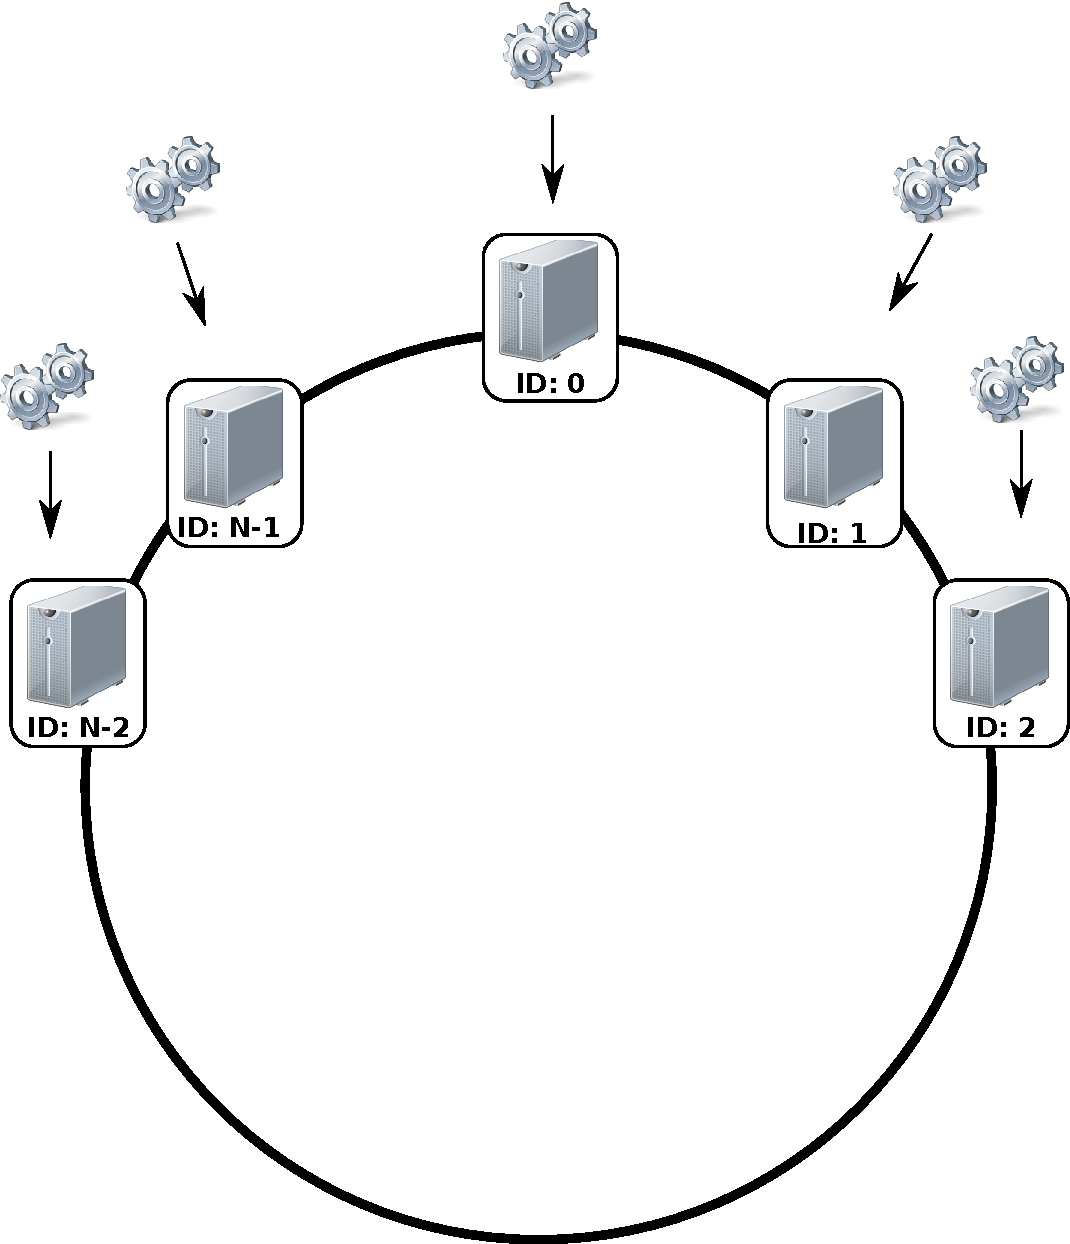
\includegraphics[width=0.8\textwidth,clip=true,trim=0px 225px 0px 0px]{resources/drawing.pdf}
\caption{A ring structured network}
\label{figring}
\end{figure}

The performance of the forwarding algorithms is measured by the average number of nodes a job must visit before being executed. The goal of the algorithms is to minimize this number by spreading the load evenly along the ring. 

\subsection{Forwarding algorithms}
Nodes that must forward a job will choose another node of the ring. Nodes have no information about other nodes, so they have no idea which nodes are idle or busy. The algorithms are grouped into two categories: forward to neighbor and forward anywhere.
The first group allows a busy node to forward an incoming job to either its left or its right neighbor, where the latter may forward these jobs to any node in the ring. 
Because the amount of dropped jobs is equal for each forwarding algorithm, these jobs will be ignored when computing the average number of forwards. One should note that the loss rate of jobs in the system is the same as the Erlang-b loss rate.

\subsection{Forward to neighbor}
\subsubsection*{Forward right}
A busy node using this technique will forward a job to its right neighbor. The job will keep traveling in this direction until an idle node is found, where it will be processed, or until it has visited all nodes when it will be dropped. Unless otherwise noted, this algorithm is used as a baseline in all further tests. This algorithm does not use any space in the job's metadata, nor must nodes save states.

\subsubsection*{Left/right forward}
A variant to the previous algorithm is the \LRF technique. Instead of forwarding each job to its right neighbor, a busy node will alternate the direction after forwarding an incoming job. To avoid a job coming back, this initial direction is saved in the job's metadata. Busy nodes receiving a job from another neighbor must forward it in the same direction as specified in the job's metadata. This algorithm requires the job to keep 1 bit representing the direction in the job's metadata, it also needs to save 1 bit state information in each node to keep track of the last direction a new job was forwarded to.

\subsubsection*{Random left/right forward with parameter $p$}
This technique is a variant of the \LRF algorithm. However, instead of alternating the direction for each new job, a node will forward a job to its right with probability $p$ and to its left with probability $1-p$. Like the previous technique, the direction is saved in the job's metadata and subsequent nodes must maintain this direction when forwarding. Unlike \LRF, nodes do not need to save state information.

\subsubsection*{Position-dependent forwarding}
As shown in figure \ref{figring}, each node in the ring has a unique ID. The IDs are ordered clockwise on the ring. Nodes using this algorithm will always forward an incoming job into the same direction: to the right when the node's id is even, to the left otherwise. Just like the previous algorithm, the direction is saved in the job's metadata and this direction must be used when other nodes have to forward the job. The initial direction of incoming jobs can be derived from the node's ID, therefore the node needs no state information.

\subsection{Forward anywhere}
The ring structure can be used in real networks, however in many cases the ring is just a virtual overlay over another structure (e.g. the internet). In these networks each node is able to connect each other node directly and more sophisticated forwarding algorithms can be used.

\subsubsection*{Random unvisited}
The Random unvisited algorithm is the most basic algorithm in this category. Every time a job must be forwarded, a list of unvisited nodes is generated and a random node is chosen from that list. The current node is added to the list of visited nodes, which is found in the job's metadata. This list can be saved using $N-1$ bits ($-1$ because the initial node is saved separately). Each unvisited node must have an equal probability of being picked.

\subsubsection*{Coprime offset}
Another algorithm is Coprime offset. This algorithm generates a list of all numbers smaller than $N$, and coprime to $N$. The first time a job is forwarded, the next number of this list is selected. This is the job's forwarding offset and it is saved in the job's metadata. When a job is forwarded, it is sent exactly this many nodes farther. Because this number and $N$ are coprime, it will visit all nodes exactly once before being returned to its originating node. 

Example:
Consider a ring size of $N=10$ in which every node is busy. The list of coprimes is: $[1, 3, 7, 9]$. Let's assume a job arrives at node $3$ and the last time node $3$ forwarded a job, the job was given offset $1$.
Because this node is busy, the next number on the list ($3$) is selected and saved in the job's metadata. All nodes are busy so the job visits all these nodes before being dropped: $3$ (arrival), $6, 9, 2, 5, 8, 1, 4, 7, 0$. Node $0$ will drop the job because the next node would be $3$, which is the node on which the job arrived.

Because the list of coprimes can be regenerated each time a job arrives, it must not be saved. Both the job and the node must keep an index to a coprime. The size of this list $\varphi(N)$, ergo an index to an element in this list requires $\lceil log_2 \varphi(N) \rceil$ bits (see section \ref{secprops} for the definition of $\varphi(N)$).

\subsubsection*{Random Coprime offset}
The Random Coprime offset algorithm is almost equal to Coprime offset. The difference between them is the decision of the offset value. Where it is the next number on the list in Coprime offset, a random value is taken from the list when using Random Coprime offset. As Coprime offset, the offset must be saved in the job's metadata. Since the offset for incoming jobs is chosen at random, the nodes do not need to keep state information.

\subsection{Properties of Algorithms}
\label{secprops}

We have reviewed some of the basic properties for each algorithm. They are summarized in table \ref{tabprops}. The function $\varphi(N)$ is Euler's totient function and counts the coprimes of $N$ up to $N$ \cite{EULER}.

\begin{eqnarray}
\varphi(N) &=& \sum_{0 < p < N, p \perp N} 1 \nonumber \\
&=&  N \cdot \prod_{p|N, p\text{ is prime}} (1-\frac{1}{p}) \nonumber
\end{eqnarray}

Note that this value is upper bound by $N-1$ and equals $N-1$ when $N$ is prime.

\footnotetext[1]{For Random Left/Right forward where $p \neq 0.5$, the probability of each path is different.}
\begin{table}[h!]
\hspace{-0.12\textwidth}
\begin{tabular}{|p{0.30\textwidth}|p{0.10\textwidth}|p{0.18\textwidth}|p{0.18\textwidth}|p{0.18\textwidth}|p{0.18\textwidth}|} \cline{2-6}
\multicolumn{1}{l|}{}		& Size known	& First forward	& Possible paths	& Space requirement (job)	& Space requirement (node) \\ \hline
Forward right				& N				& 1				& 1					& 0							& 0		\\ \hline
Left/right forward			& N				& 2				& 2					& 1							& 1		\\ \hline
Random left/right forward (p) & N			& 2				& 2 $^($\footnotemark$^)$ & 1					& 0		\\ \hline
Position dependent forward	& N				& 1				& 1					& 1							& 0		\\ \hline
Random unvisited			& Y				& $N-1$			& $(N-1)!$			& $N-1$	& 0		\\ \hline
Coprime offset				& Y				& $\varphi(N)$		& $\varphi(N)$ 		& $\lceil log_2 \varphi(N) \rceil$	& $\lceil log_2 \varphi(N) \rceil$ \\ \hline
Random coprime offset		& Y				& $\varphi(N)$		& $\varphi(N)$			& $\lceil log_2 \varphi(N) \rceil$	& 0		\\ \hline
\end{tabular}
\caption{Properties of forwarding algorithms}
\label{tabprops}
\end{table}

\begin{description}
\item[Size known] Represents whether the size of the ring must be known to the nodes in order for the algorithm to function. This implies that a change in the ring (node joins or leaves) must be propagated over the ring.
\item[First forward] When the node on which the incoming job arrives is busy, this number represents the number of candidates to which the node can forward the job.
\item[Possible paths] Assuming the system is saturated, this number represents the number of possible paths a job can travel until being dropped. The probability of each path is the same (unless otherwise noted).
\item[Space requirement (job)] This value represents the number of bits required in the job's metadata.
\item[Space requirement (node)] This value represents the number of bits required to save the node's state information.
\end{description}

\section{Simulation}
\label{secsimulation}
To evaluate the different algorithms discussed in the previous section, 2 methods will be used. Our first method is using a simulator. The second method is the numerical evaluation of the simulation results using MATLAB. The validation method is further discussed in section \ref{secvalidation}.

The simulation is accomplished using a custom simulator. A continuous time simulator is written in C++, using no external requirements but the STL and OpenMP \cite{OPENMP}. The source code of the simulator can be found in appendix \ref{sourcecode} or at \url{http://code.google.com/p/powerofpaths/}.

The simulator can be controlled using a command line interface of which the usage is described below:
\lstset{language=sh,caption={Simulator usage description}}
\begin{lstlisting}
Usage: -r -s long -j double -a double -n long -p long -l long -t long -h type
	-r	Random seed
	-s	Set seed			(default: 0)
	-j	Job length			(default: 1.0)
	-a	Load				(default: 1.0)
	-n	Ring size			(default: 100)
	-c	Processing units per node	(default: 1)
	-p	Print progress interval		(default: -1 - disabled)
	-l	Simulation length		(default: 3600)
	-t	Repetition			(default: 1)
	-h	Print this help
	 type	right | switch | randswitch | evenswitch | prime | randprime | randunvisited | totop
\end{lstlisting}

\subsection{Measure}
The goal of the algorithms is to distribute the jobs evenly along the ring. This implies that the number of nodes a job must visit should be low. As a measure for our experiments, we will be using the average number of times a job is forwarded before it is executed. Since the number of forwards of a job that could not be executed is the same for each algorithm (i.e. $N-1$: traversing each link but one), and the loss rate of each algorithm is the same (because forwards are instantaneous), we will not take these dropped jobs into account when computing the average.

It is clear that when the system load approaches $0$, the probability that a node is busy will also approach $0$ and the average number of forwards will therefore also approach $0$. On the other hand, when the load approaches $\infty$, each node's probability of being busy will approach $1$ and therefore the number of forwards will be $N-1$ and the job will fail. A system with load $> 1$ is called an overloaded system. For the purpose of this thesis, only loads up to $1$ are discussed.

We will compare each algorithm to a baseline result. The baseline used in this thesis is the \FR algorithm. This means that each graph will show its result relative to the \FR results. The results given by the simulator were obtained using a ring size of 100 and using a random seed for each run.

The absolute performance of the baseline algorithm is shown in figure \ref{baseline}.

\begin{figure}[h!tb]
\centering
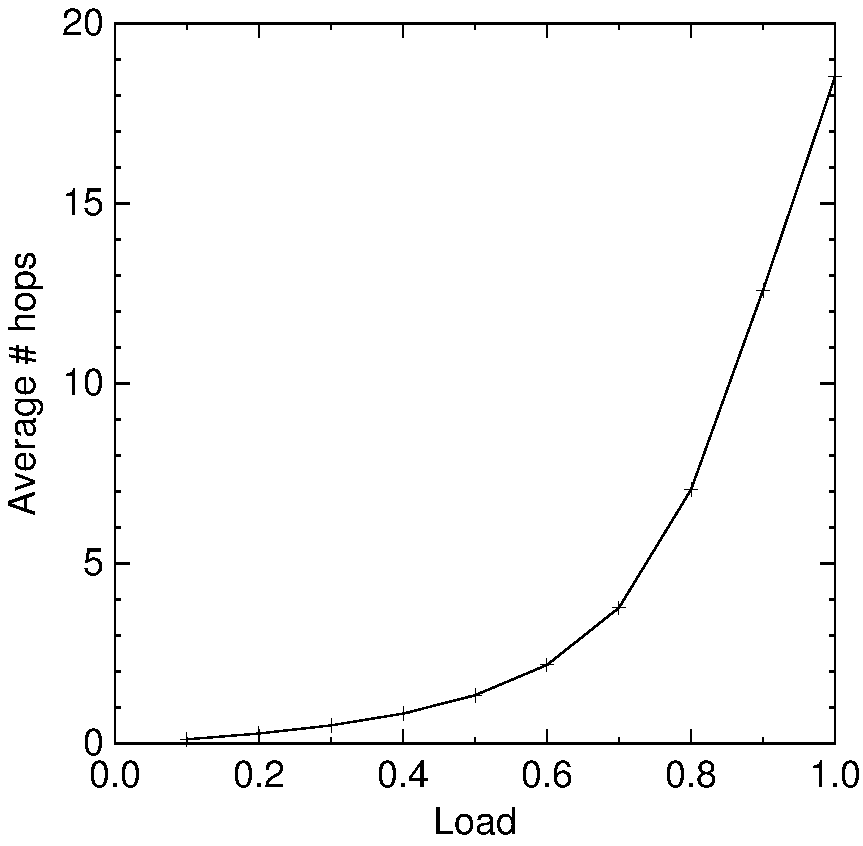
\includegraphics[width=0.6\textwidth]{data/right.pdf}
\caption{The forward right baseline result}
\label{baseline}
\end{figure}

\subsection{Results}
\label{simresults}

\subsubsection*{Left/right forward}
It is intuitively clear that alternating the forwarding direction of incoming jobs should distribute the load better than keeping the same direction, certainly under temporary local heavy load. Figure \ref{figlr} shows the improvement made by the \LRF algorithm over the \FR method. The performance gain is at least 1\% and up to over 4\% under medium load.

\begin{figure}[h!tb]
\centering
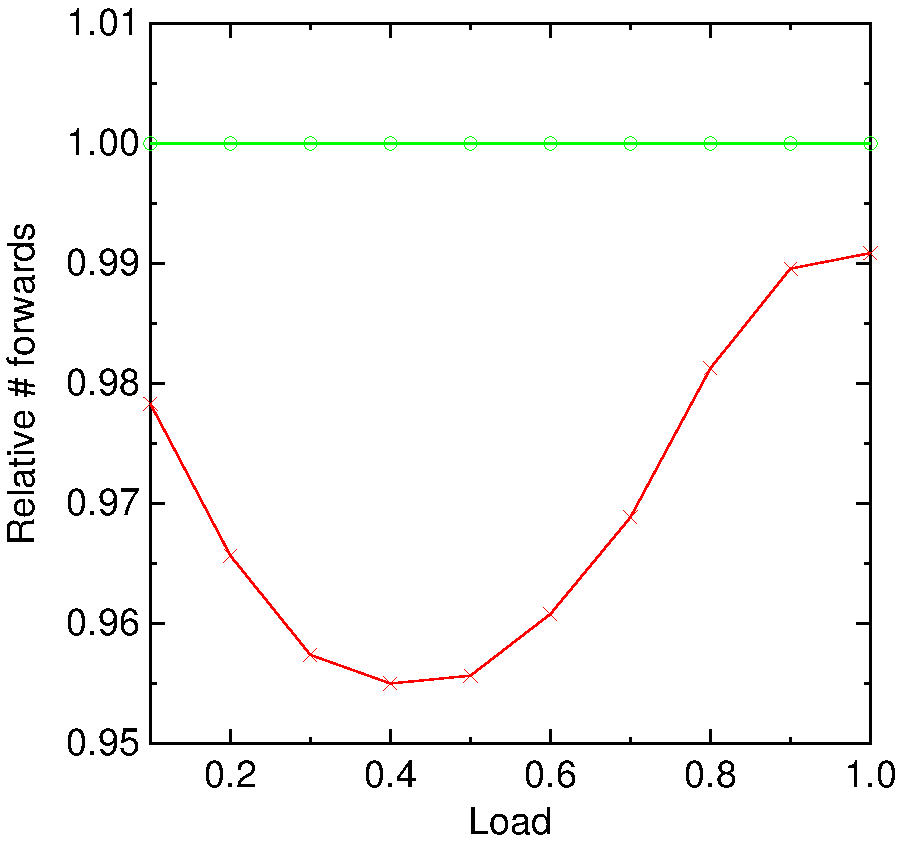
\includegraphics[width=0.6\textwidth]{data/switchright.pdf}
\caption{Left/right forward}
\label{figlr}
\end{figure}


\subsubsection*{Random left/right forward with parameter $p$}
For $p=0.5$, one would expect the results of this algorithm being similar to those obtained in the previous simulation. However, it seems the small change in the algorithm worsened the results significantly.

\begin{figure}[h!tb]
\centering
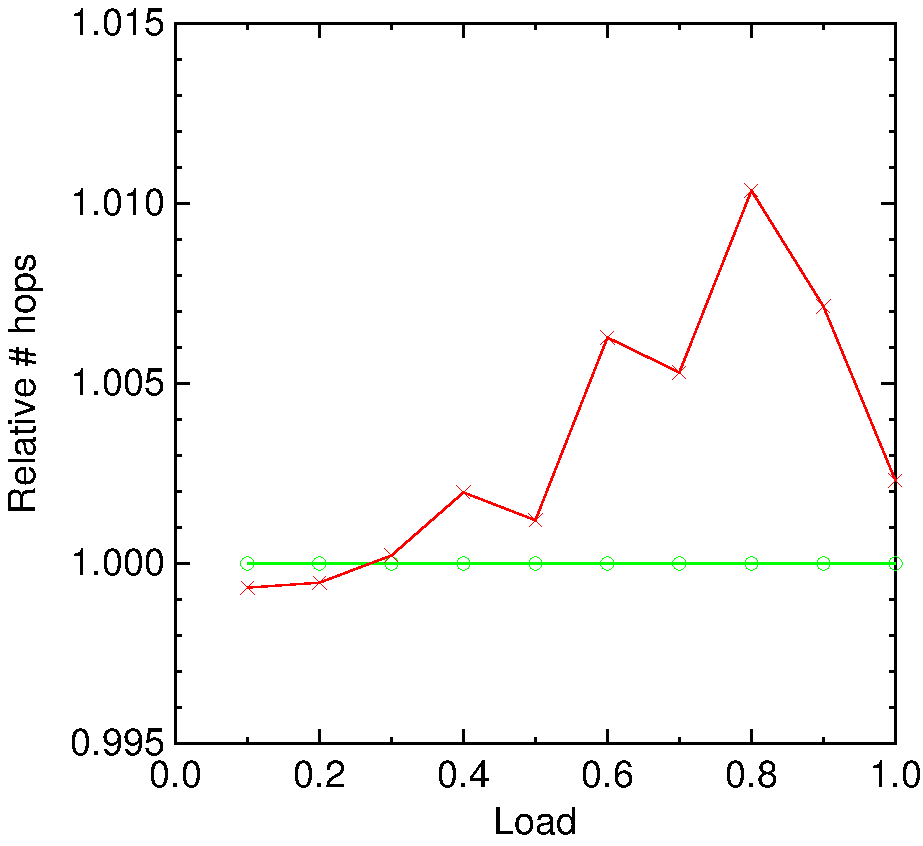
\includegraphics[width=0.6\textwidth]{data/randswitchright.pdf}
\caption{Random Left/Right forward with parameter $0.5$}
\label{figrandswitch}
\end{figure}

Figure \ref{figrandswitch} shows the results of this algorithm for $p=0.5$. For $p=0$, the algorithm is equal to the \FR algorithm. Hence, we should investigate how different values of $p$ influence the final results. Figure \ref{figrandswitchp} shows the results obtained for $0 \leq p \leq 0.5$. We find no value of $p$ for which this algorithm performs better than \FR.

\begin{figure}[h!tb]
\centering
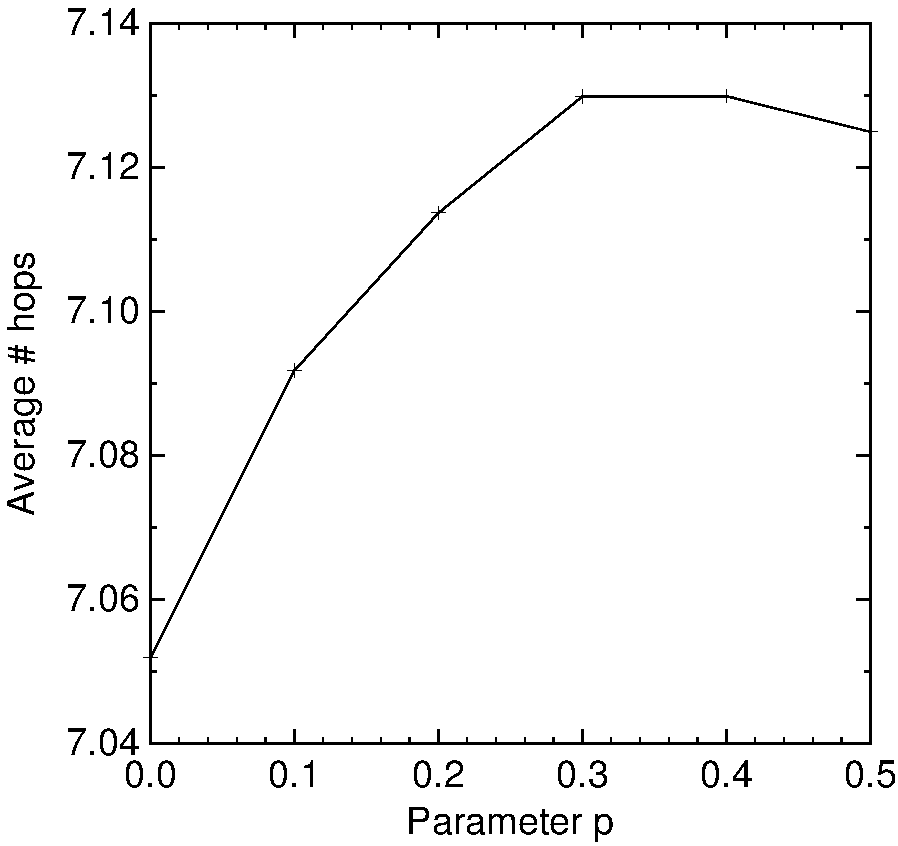
\includegraphics[width=0.6\textwidth]{data/randswitchp.pdf}
\caption{Random Left/Right forward with load $0.8$}
\label{figrandswitchp}
\end{figure}

\subsubsection*{Position-dependant forwarding}
This technique groups every 2 nodes into small virtual clusters. When a job arrives at a busy node, the job will be forwarded to the other node in this cluster. Jobs leaving a cluster will seem to do this in a random direction ($p=0.5$). Since the load is concentrated per cluster instead of being distributed over the whole system, this technique performs worse than other techniques. The results are shown in figure \ref{figevenswitch}.

\begin{figure}[h!tb]
\centering
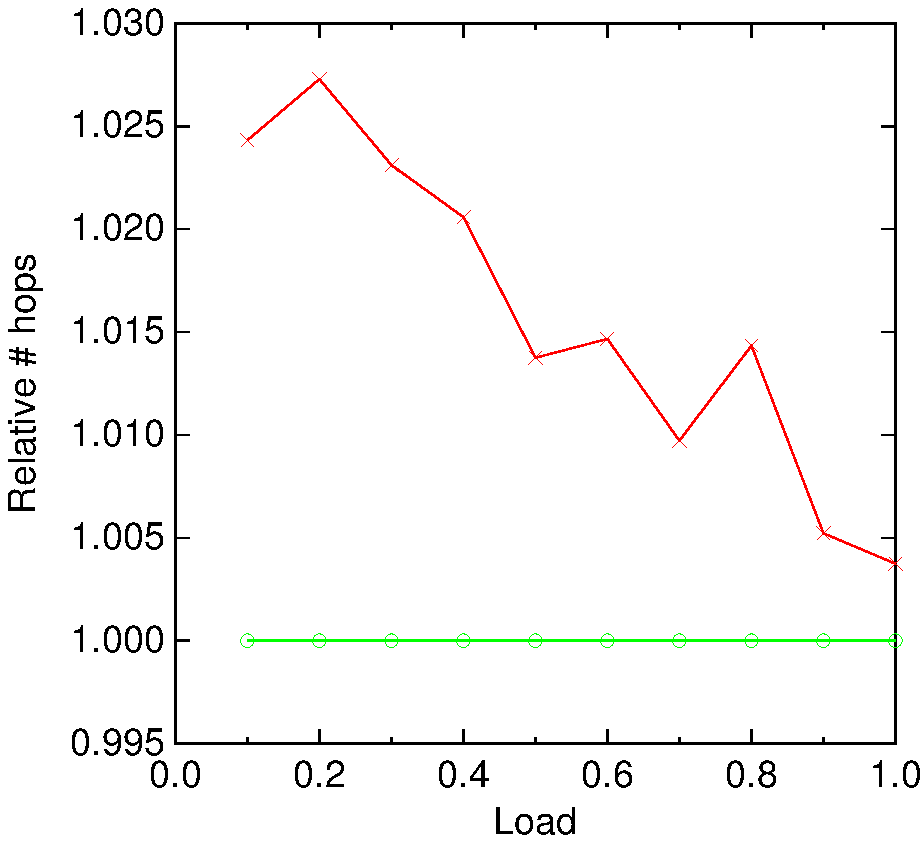
\includegraphics[width=0.6\textwidth]{data/evenswitchright.pdf}
\caption{Position-dependant forwarding}
\label{figevenswitch}
\end{figure}


\subsubsection*{Random unvisited}
Unlike the previous algorithms, this algorithm is not bound to its neighbors when forwarding a job. Lifting this constraint allows a serious performance boost.

\begin{figure}[h!tb]
\centering
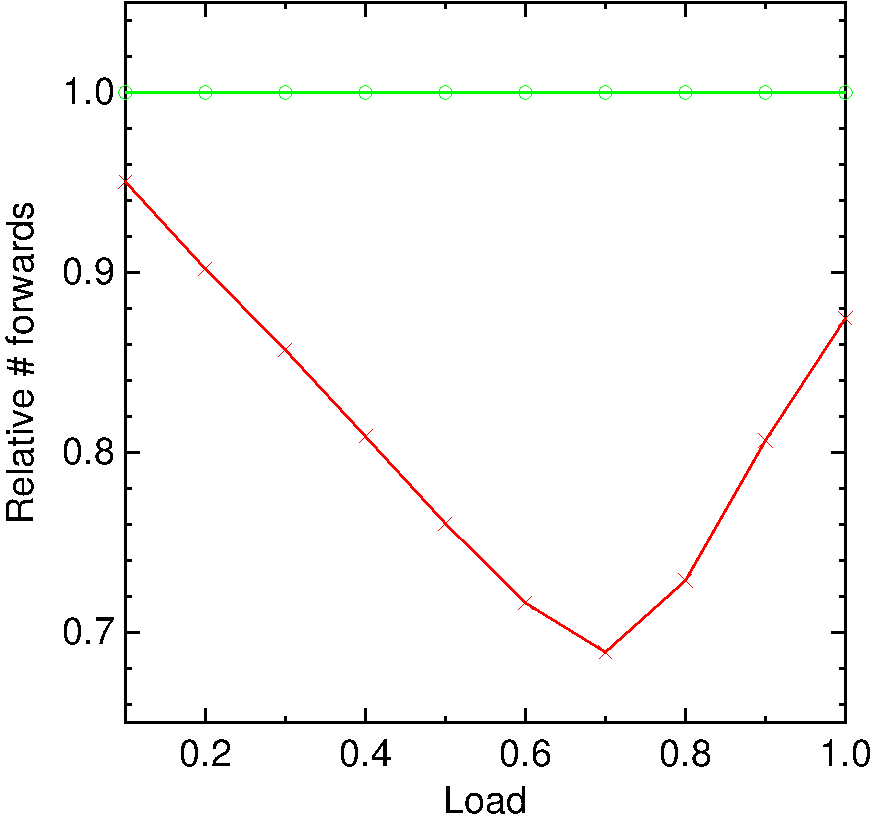
\includegraphics[width=0.6\textwidth]{data/randunvisitedright.pdf}
\caption{Random unvisited forwarding}
\label{figrandunvisited}
\end{figure}

Figure \ref{figrandunvisited} shows the results of this algorithm. The performance benefit is at least $10 \%$ in the range $0.20 - 1.00$, and even up to $30 \%$ under medium load.

\subsubsection*{(Random) Coprime offset}
Two other algorithms that are not restricted to forwarding to a neighbor are Coprime offset and Random coprime offset. Figure \ref{figprimes} shows the results of both these algorithms. The difference of these algorithms with themselves and the random unvisited algorithms is not clearly visible when comparing both to the \FR algorithm. To put these results in perspective, we included figure \ref{figrurrp} where Coprime offset and Random Coprime offset are depicted relative to Random unvisited. Although the difference is very small, it seems the Random unvisited algorithm shows a better performance than the other two. However, Coprime offset and Random Coprime offset require $\lceil log_2 \varphi(N) \rceil$ bits in the job's metadata instead of $N$ for Random unvisited.

\begin{figure}[h!tb]
        \begin{subfigure}[b]{0.5\textwidth}
                \centering
                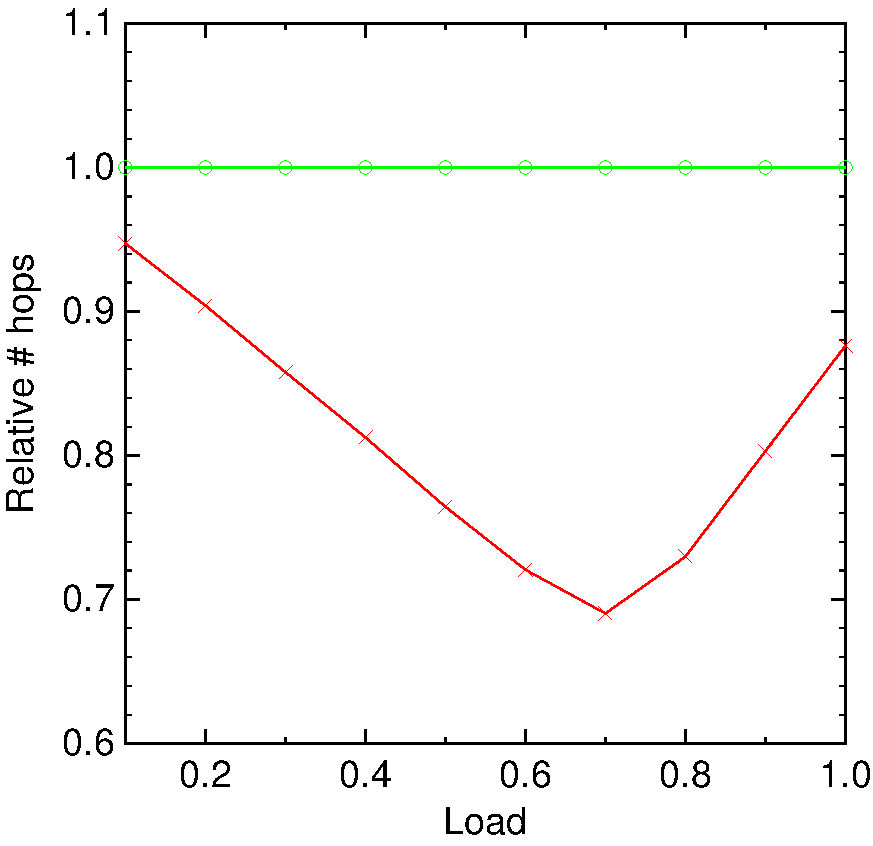
\includegraphics[width=\textwidth]{data/primeright.pdf}
                \caption{Coprime offset}
        \end{subfigure}
        \begin{subfigure}[b]{0.5\textwidth}
                \centering
                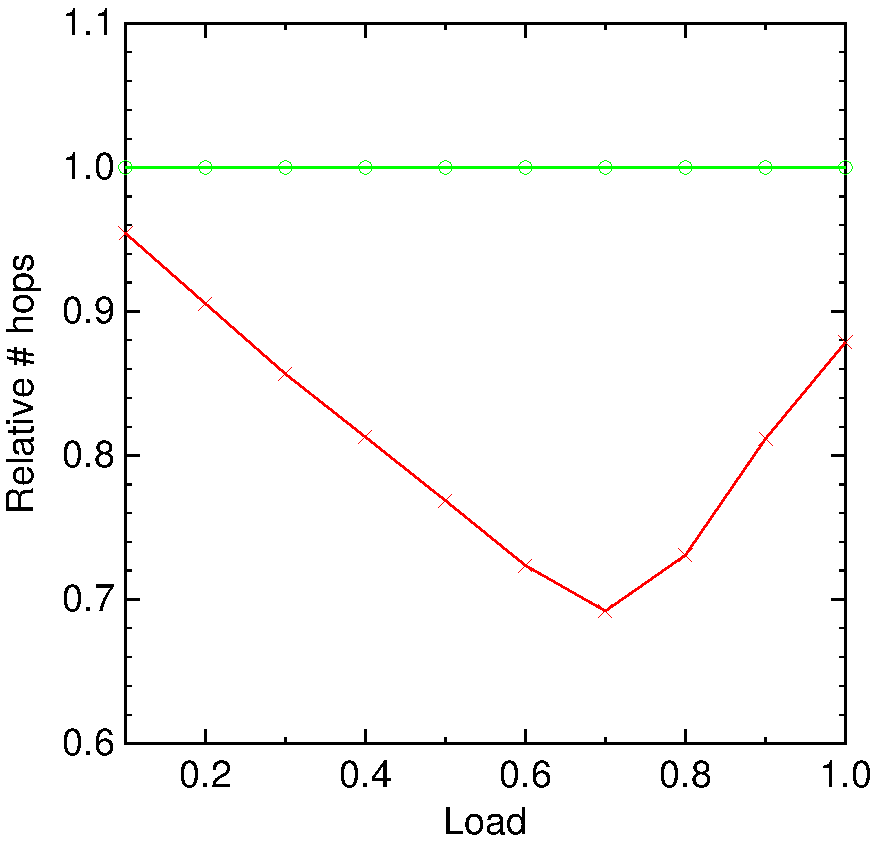
\includegraphics[width=\textwidth]{data/randprimeright.pdf}
                \caption{Random Coprime offset}
                \label{figsimrcp}
        \end{subfigure}
\caption{(Random) Coprime offset}
\label{figprimes}
\end{figure}

\begin{figure}[h!tb]
\centering
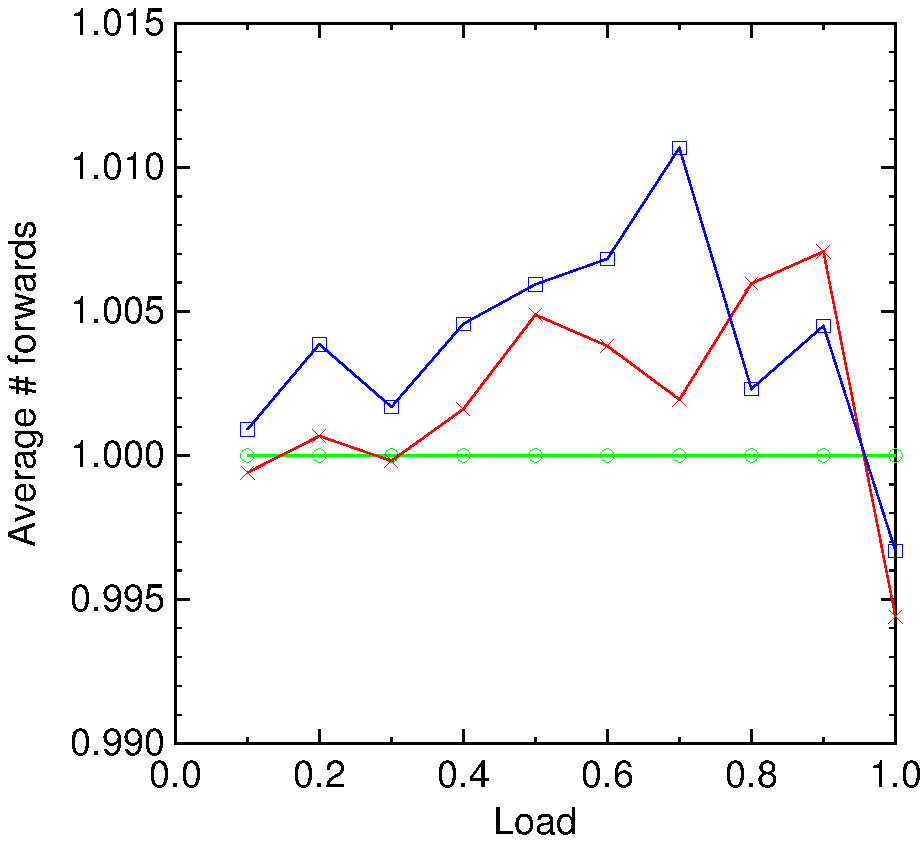
\includegraphics[width=0.8\textwidth]{data/randunvisited_prime_randprime.pdf}
\caption{Random unvisited (green), Coprime offset (blue), Random Coprime offset (Red)}
\label{figrurrp}
\end{figure}



\subsection{Multiple execution units}
So far, all simulations were executed using 1 CPU per server. This is not a realistic assumption for most distributed systems. This section is intended to research the behavior of the algorithms when using multiple CPUs, and comparing the results to a system with 1 CPU per server, and to each other.

Per algorithm, two simulations were performed and compared. One using 1 CPU per server and one using 4 CPUs per server. See table \ref{tabcpus} for more information about the tests.

\begin{table}[h!]
\centering
\begin{tabular}{|p{0.3\textwidth}|p{0.35\textwidth}|p{0.35\textwidth}|} \hline
Algorithms & \multicolumn{2}{|p{0.7\textwidth}|}{Forward right, Left/right forward, Random left/right (0.5), Random unvisited, Random coprime offset} \\ \hline
Ring size & 100 & 25 \\ \hline
CPUs per node	& 1 & 4 \\ \hline
Total CPUs in system & \multicolumn{2}{|c|}{100} \\ \hline
Load	& \multicolumn{2}{|c|}{$0.1 - 1.0$} \\ \hline
\end{tabular}
\caption{Comparison of algorithms using multiple CPUs per server}
\label{tabcpus}
\end{table}

Since the ring size for the second test is 25 instead of 100, the number of forwards of the second test will be multiplied by 4 to get meaningful results. This actually makes sense because a job that is forwarded once has encountered 4 busy CPUs. The baseline for the tests is the result of the algorithm using 1 CPU (found in section \ref{simresults}), where the results of the simulation using multiple CPUs is drawn relative to the baseline result.

\begin{figure}
        \begin{subfigure}[b]{0.5\textwidth}
                \centering
                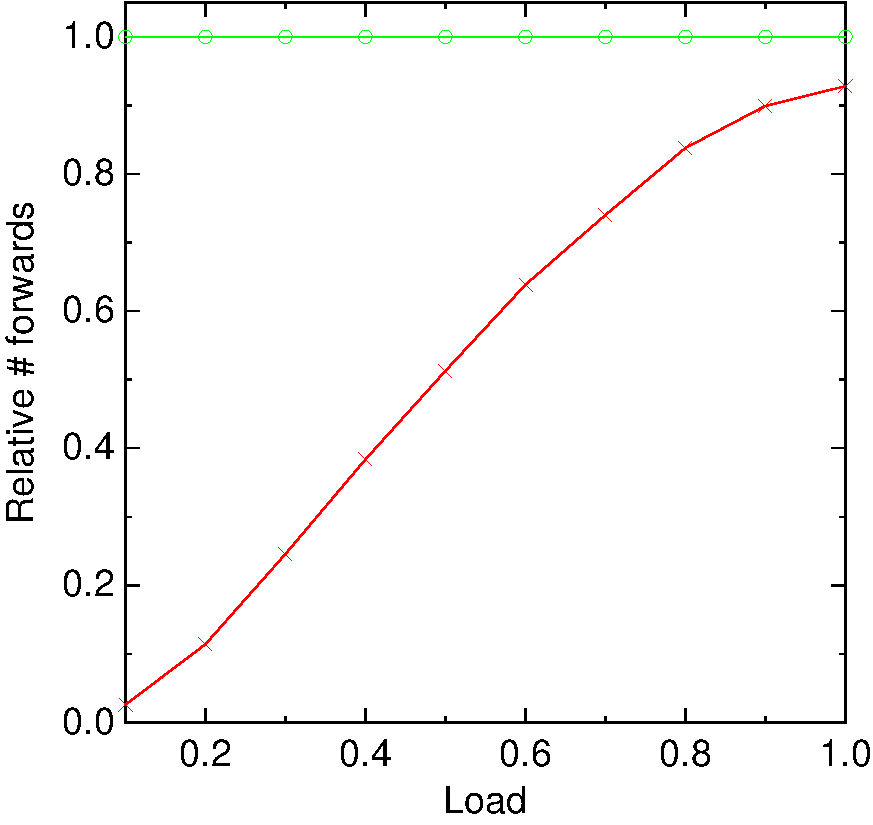
\includegraphics[width=\textwidth]{data/4rightright.pdf}
                \caption{Forward right}
        \end{subfigure}
        \begin{subfigure}[b]{0.5\textwidth}
                \centering
                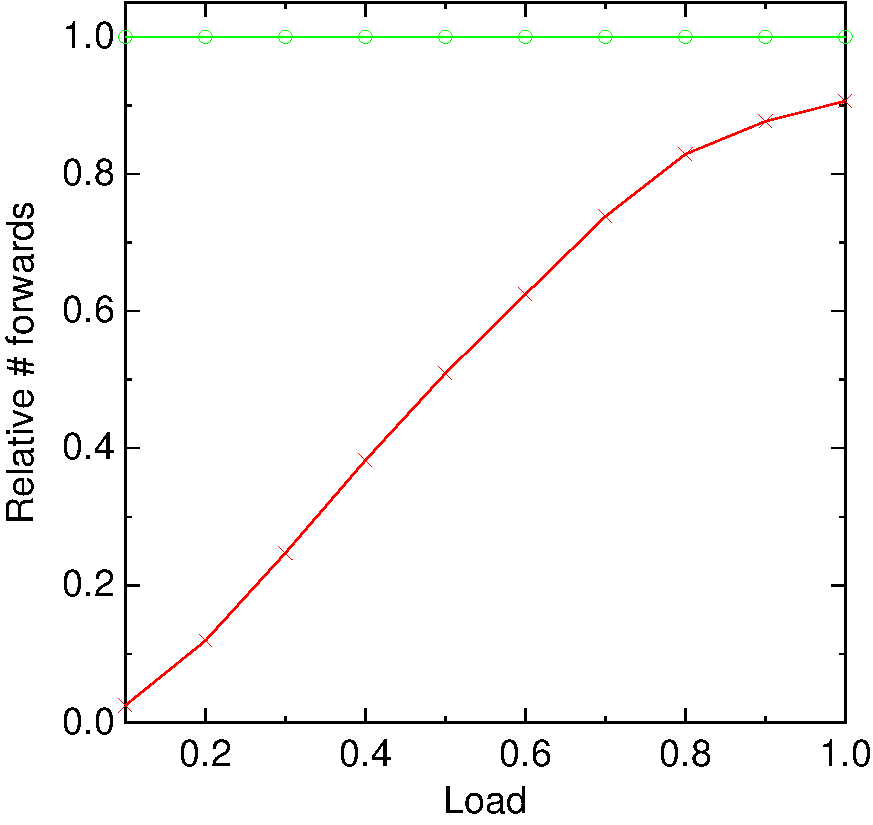
\includegraphics[width=\textwidth]{data/4switchswitch.pdf}
                \caption{Left/right forward}
        \end{subfigure}

        \vspace*{1.6em}

        \begin{subfigure}[b]{0.5\textwidth}
                \centering
                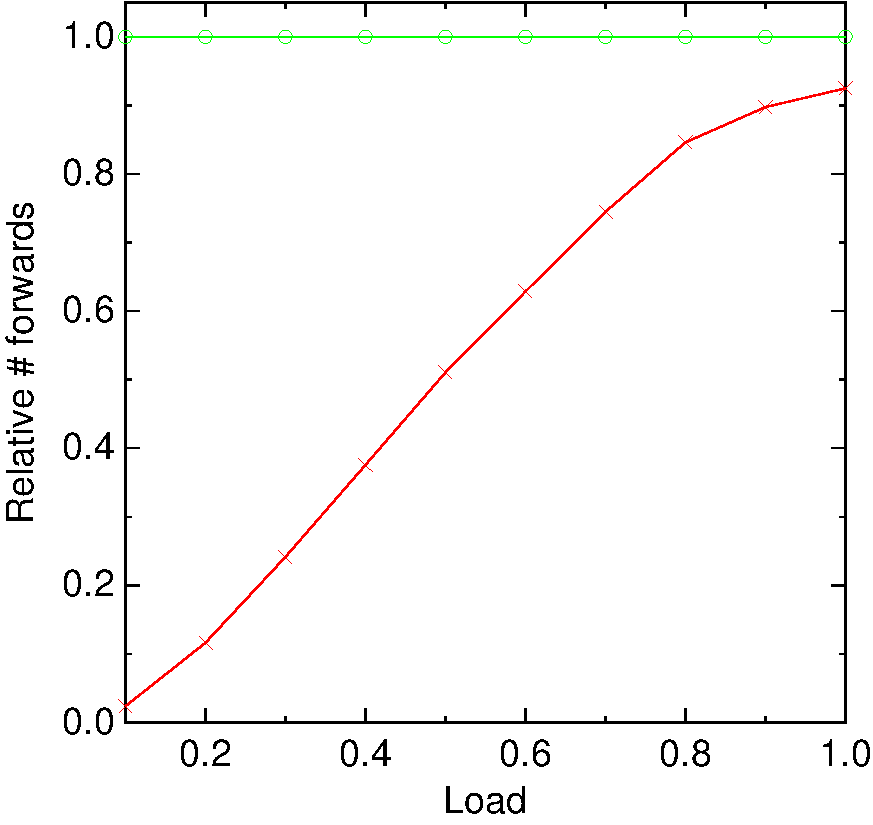
\includegraphics[width=\textwidth]{data/4randswitchrandswitch.pdf}
                \caption{Random left/right forward (0.5)}
        \end{subfigure}
        \begin{subfigure}[b]{0.5\textwidth}
                \centering
                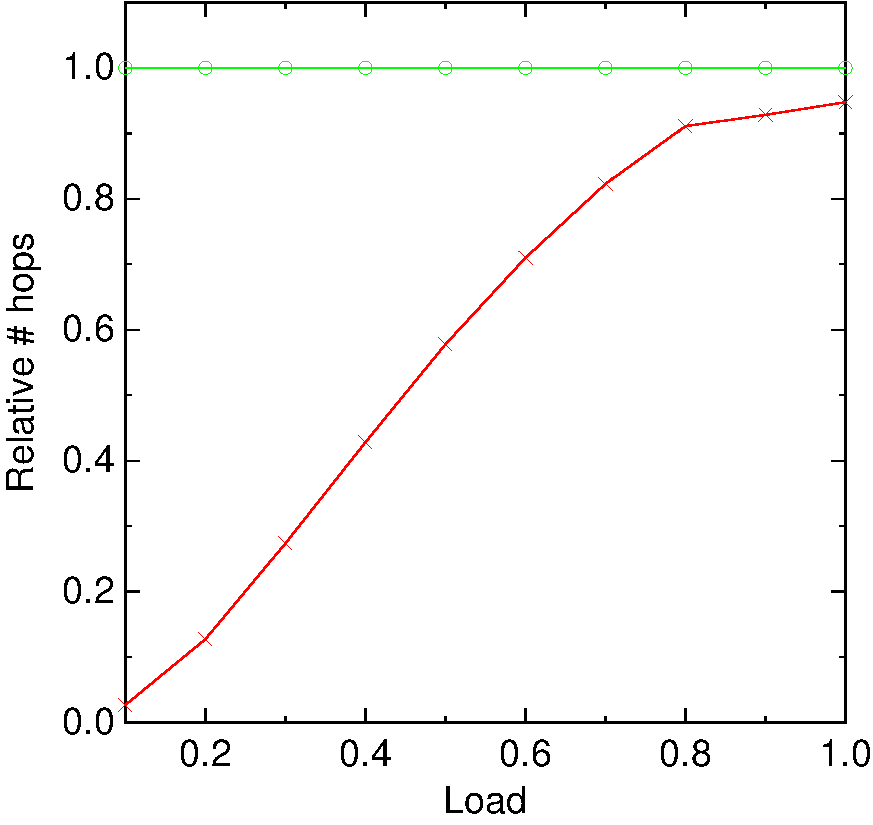
\includegraphics[width=\textwidth]{data/4randunvisitedrandunvisited.pdf}
                \caption{Random unvisited}
        \end{subfigure}

        \vspace*{1.6em}

        \begin{subfigure}[b]{0.5\textwidth}
                \centering
                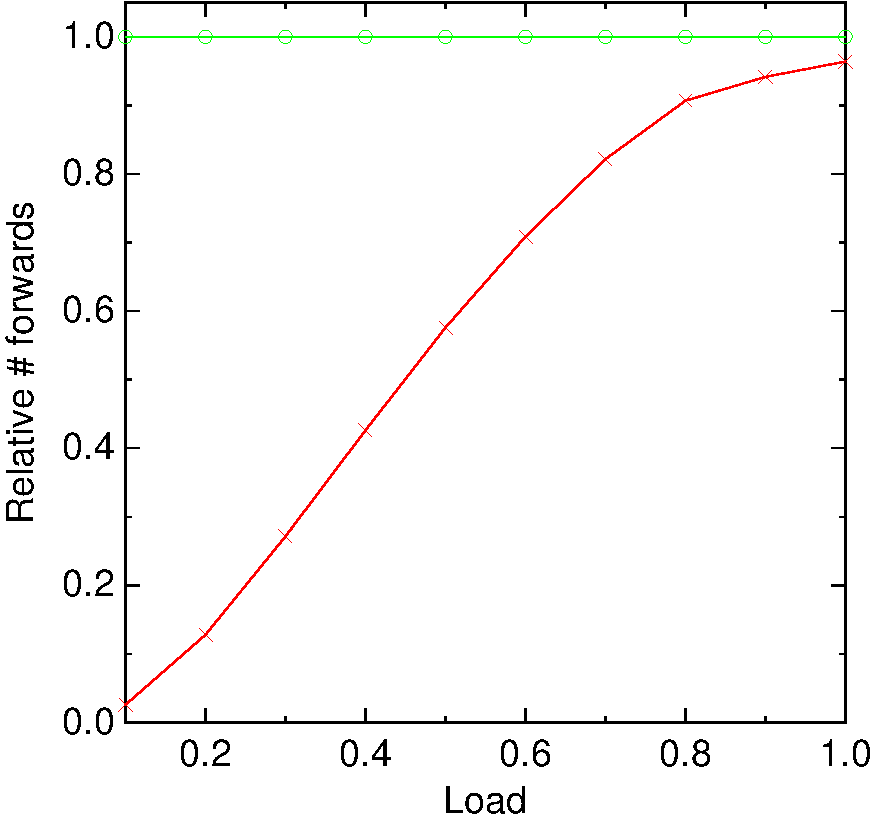
\includegraphics[width=\textwidth]{data/4randprimerandprime.pdf}
                \caption{Random coprime offset}
        \end{subfigure}
        \caption{4 CPUs per server versus 1}\label{figcpus}
\end{figure}

Figure \ref{figcpus} shows the performance of 4 CPUs versus 1 CPU for different algorithms. For each tested algorithm, we obtain the same result. This means the results of each algorithm are influenced in the same way when using multiple CPUs per server. We can use this knowledge to generalize the results of section \ref{simresults}.

Since we assume each algorithm is influenced the same way, we will investigate one of them in depth. We will try to transform the results of an algorithm with ring size $N$ and $1$ CPU per server into the results of the same algorithm with ring size $N/c$ and $c$ CPUs per server. Every other parameter should be unchanged.

Let $d$ be the distribution of the number of forwards, stored as a row vector. We will build a transformation vector $M$ in the form $[ \lfloor 0/c \rfloor,  \lfloor 1/c \rfloor, \ldots, \lfloor (N-1)/c \rfloor]'$. This vector represents the number of times a job would be forwarded if there would be $c$ CPUs per server. $d*M$ equals the average number of forwards when using such a system. To ignore the dropped jobs, the results must be weighted for only the completed jobs.
In our example, we will transform the results of the \FR algorithm using ring size $N=10$ and 1 CPU into the results of a ring with size $N=5$ and $c=2$ CPUs per server, see table \ref{tabdistr} for a worked out example and figure \ref{figcpusmatch} for a comparison of the transformation and a simulation result.


\begin{table}
\centering
\begin{tabular}{|r|l|r|l|} \hline
\# hops & Distribution & M & Result \\ \hline
0 & 0.5092 & 0 & 0 \\ \hline
1 & 0.2118 & 0 & 0 \\ \hline
2 & 0.1082 & 1 & 0.1082 \\ \hline
3 & 0.0609 & 1 & 0.0609 \\ \hline
4 & 0.0363 & 2 & 0.0726 \\ \hline
5 & 0.0224 & 2 & 0.0449 \\ \hline
6 & 0.0142 & 3 & 0.0426 \\ \hline
7 & 0.0091 & 3 & 0.0272 \\ \hline
8 & 0.0058 & 4 & 0.0233 \\ \hline
9 & 0.0037 & 4 & 0.0147 \\ \hline
Total &  0.9816 & &  0.3944 \\ \hline
Weighted total & \multicolumn{3}{|c|}{$0.3944/0.9816 = 0.4018 $} \\ \hline
Simulation result & \multicolumn{3}{|c|}{$0.4171$} \\ \hline
\end{tabular}
\caption{Comparison when load=0.5}
\label{tabdistr}
\end{table}

\begin{figure}[h!tb]
\centering
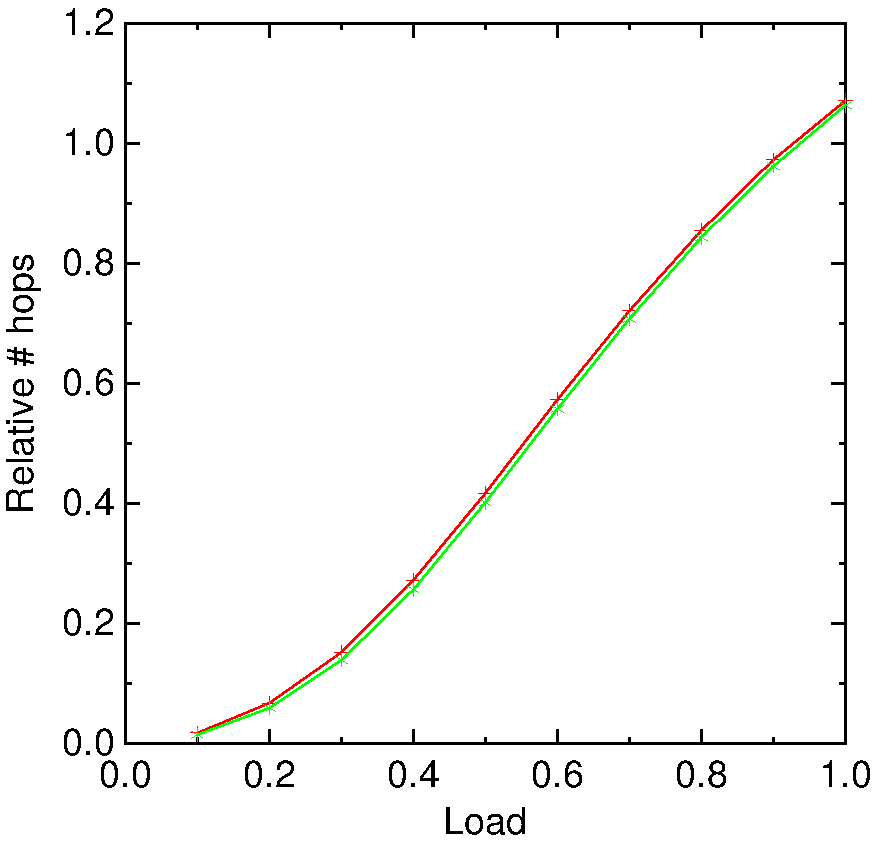
\includegraphics[width=0.8\textwidth]{data/right_5_2.pdf}
\caption{Multiple CPUs result derived of the result for 1 CPU (green) versus an actual simulation result using 4 CPUs (red)}
\label{figcpusmatch}
\end{figure}

While deriving the transformation, we did not take into account that for each choice the algorithm makes, $c$ CPUs are bound to this choice. The real simulation chooses a node and must first test all those CPUs where the transformation only counts the $n \cdot c$ forwards using a better choice for each forward. This makes the transformation nothing more than an approximation and an upper bound of the real results.

\section{Numerical Validation}
\label{secvalidation}

To validate the results obtained in the previous section, we modeled the scheduling algorithms into Markov Chains. Using the steady state distribution of these chains, we can derive the average number of hops and the average loss.
For $N$ nodes in a ring, the Markov chain consists of $2^N$ states, where the $n$-th bit represents whether the $n$-th server is busy ($1$) or idle ($0$). To optimize the computation time and memory requirements, we used sparse matrices for the validation. The validation code is written in MATLAB, it can be found in appendix \ref{matlabcode} or on \url{http://code.google.com/p/powerofpaths/}.

The validation of the results happens in a different environment than the simulation. Because of the non-polynomial execution time of the algorithm, the size of the ring is reduced to $10$. Therefore, the results of this validation are smaller but the relative results are still relevant.

Not every algorithm can be modeled efficiently into a Markov Chain. Computing the results of algorithms requiring state information in the nodes is infeasible for a decent ring size, therefore we did not model \LRF and the Coprime offset algorithms. We also ignored the Position dependant forwarding algorithm since its results seemed logical and further investigation would not reveal useful information.

\subsection{Comparison}
\subsubsection*{Forward right}
Modeling a technique into a Markov Chain is an easy operation for most algorithms. The example given below is for a ring of 3 nodes. For convenience, the states are represented in their binary form.

\[ Q =
  \begin{blockarray}{ccccccccc}
    & 000 & 001 & 010 & 011 & 100 & 101 & 110 & 111 \\
    \begin{block}{c[cccccccc]}
    000 & -3 \lambda & \lambda & \lambda & 0 & \lambda & 0 & 0 & 0 \\
    001 & \mu & -3\lambda-\mu & 0 & \lambda & 0 & 2\lambda & 0 & 0 \\
    010 & \mu & 0 & -3\lambda-\mu & 2\lambda & 0 & 0 & \lambda & 0 \\
    011 & 0 & \mu & \mu & -3\lambda-2\mu & 0 & 0 & 0 & 3\lambda \\
    100 & \mu & 0 & 0 & 0 & -3\lambda-\mu & \lambda & 2\lambda & 0 \\
    101 & 0 & \mu & 0 & 0 & \mu & -3\lambda-2\mu & 0 & 3\lambda \\
    110 & 0 & 0 & \mu & 0 & \mu & 0 & -3\lambda-2\mu & 3\lambda \\
    111 & 0 & 0 & 0 & \mu & 0 & \mu & \mu & -3\mu \\
    \end{block}
  \end{blockarray}
\]

\begin{figure}[h!tb]
\centering
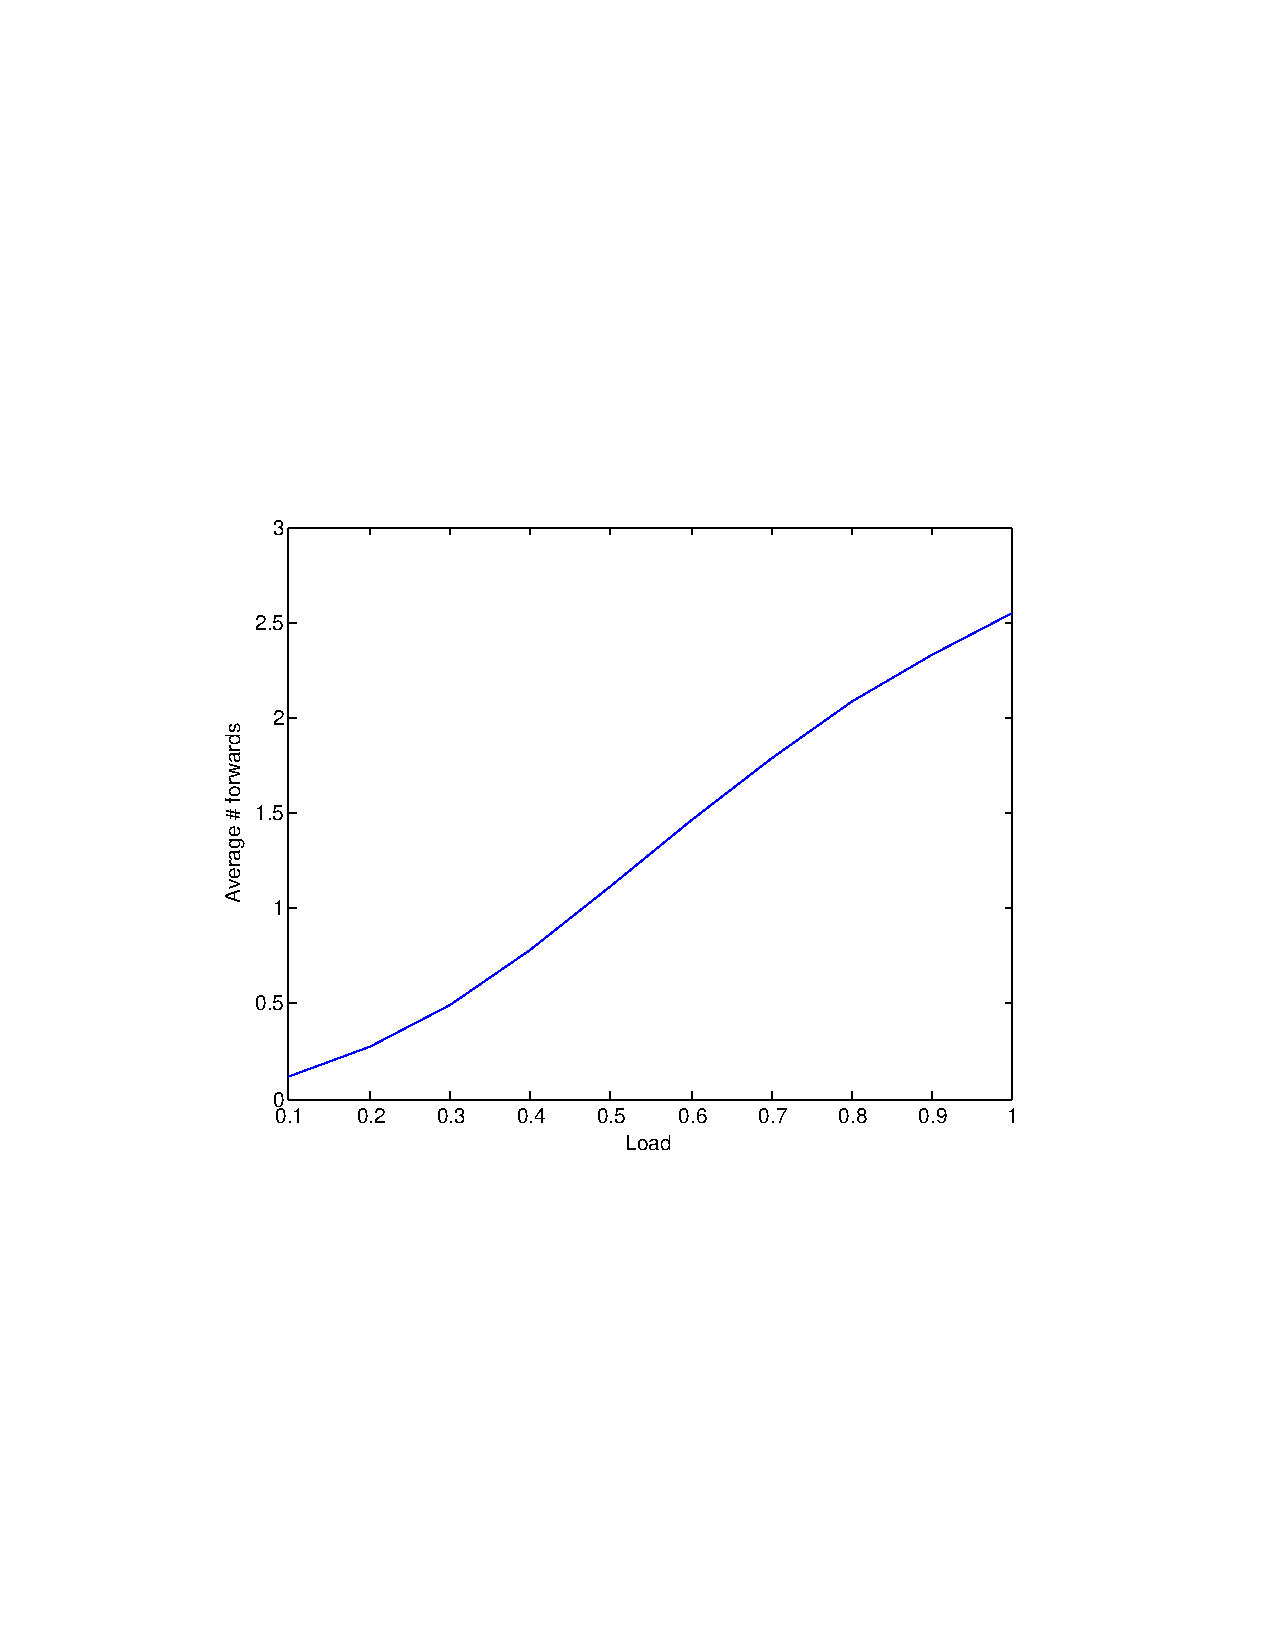
\includegraphics[clip=true, trim=9em 24em 9em 24em, width=0.9\textwidth]{resources/plotright.pdf}
\caption{Validation of forward right}
\label{validright}
\end{figure}

Like to the simulation section, this method will be the baseline result in our other results.

\subsubsection*{Random left/right forward with parameter $p$}
This matrix is very similar to the one above. But we need to take into account the parameters $p$ and $1-p$ instead of $1$ and $0$.

\[ Q =
  \begin{blockarray}{ccccccccc}
    & 000 & 001 & 010 & 011 & 100 & 101 & 110 & 111 \\
    \begin{block}{c[cccccccc]}
    000 & -3 \lambda & \lambda & \lambda & 0 & \lambda & 0 & 0 & 0 \\
    001 & \mu & -3\lambda-\mu & 0 & (2-p)\lambda & 0 & (1+p)\lambda & 0 & 0 \\
    010 & \mu & 0 & -3\lambda-\mu & (1+p)\lambda & 0 & 0 & (2-p)\lambda & 0 \\
    011 & 0 & \mu & \mu & -3\lambda-2\mu & 0 & 0 & 0 & 3\lambda \\
    100 & \mu & 0 & 0 & 0 & -3\lambda-\mu & (2-p)\lambda & (1+p)\lambda & 0 \\
    101 & 0 & \mu & 0 & 0 & \mu & -3\lambda-2\mu & 0 & 3\lambda \\
    110 & 0 & 0 & \mu & 0 & \mu & 0 & -3\lambda-2\mu & 3\lambda \\
    111 & 0 & 0 & 0 & \mu & 0 & \mu & \mu & -3\mu \\
    \end{block}
  \end{blockarray}
\]

\begin{figure}[h!tb]
\centering
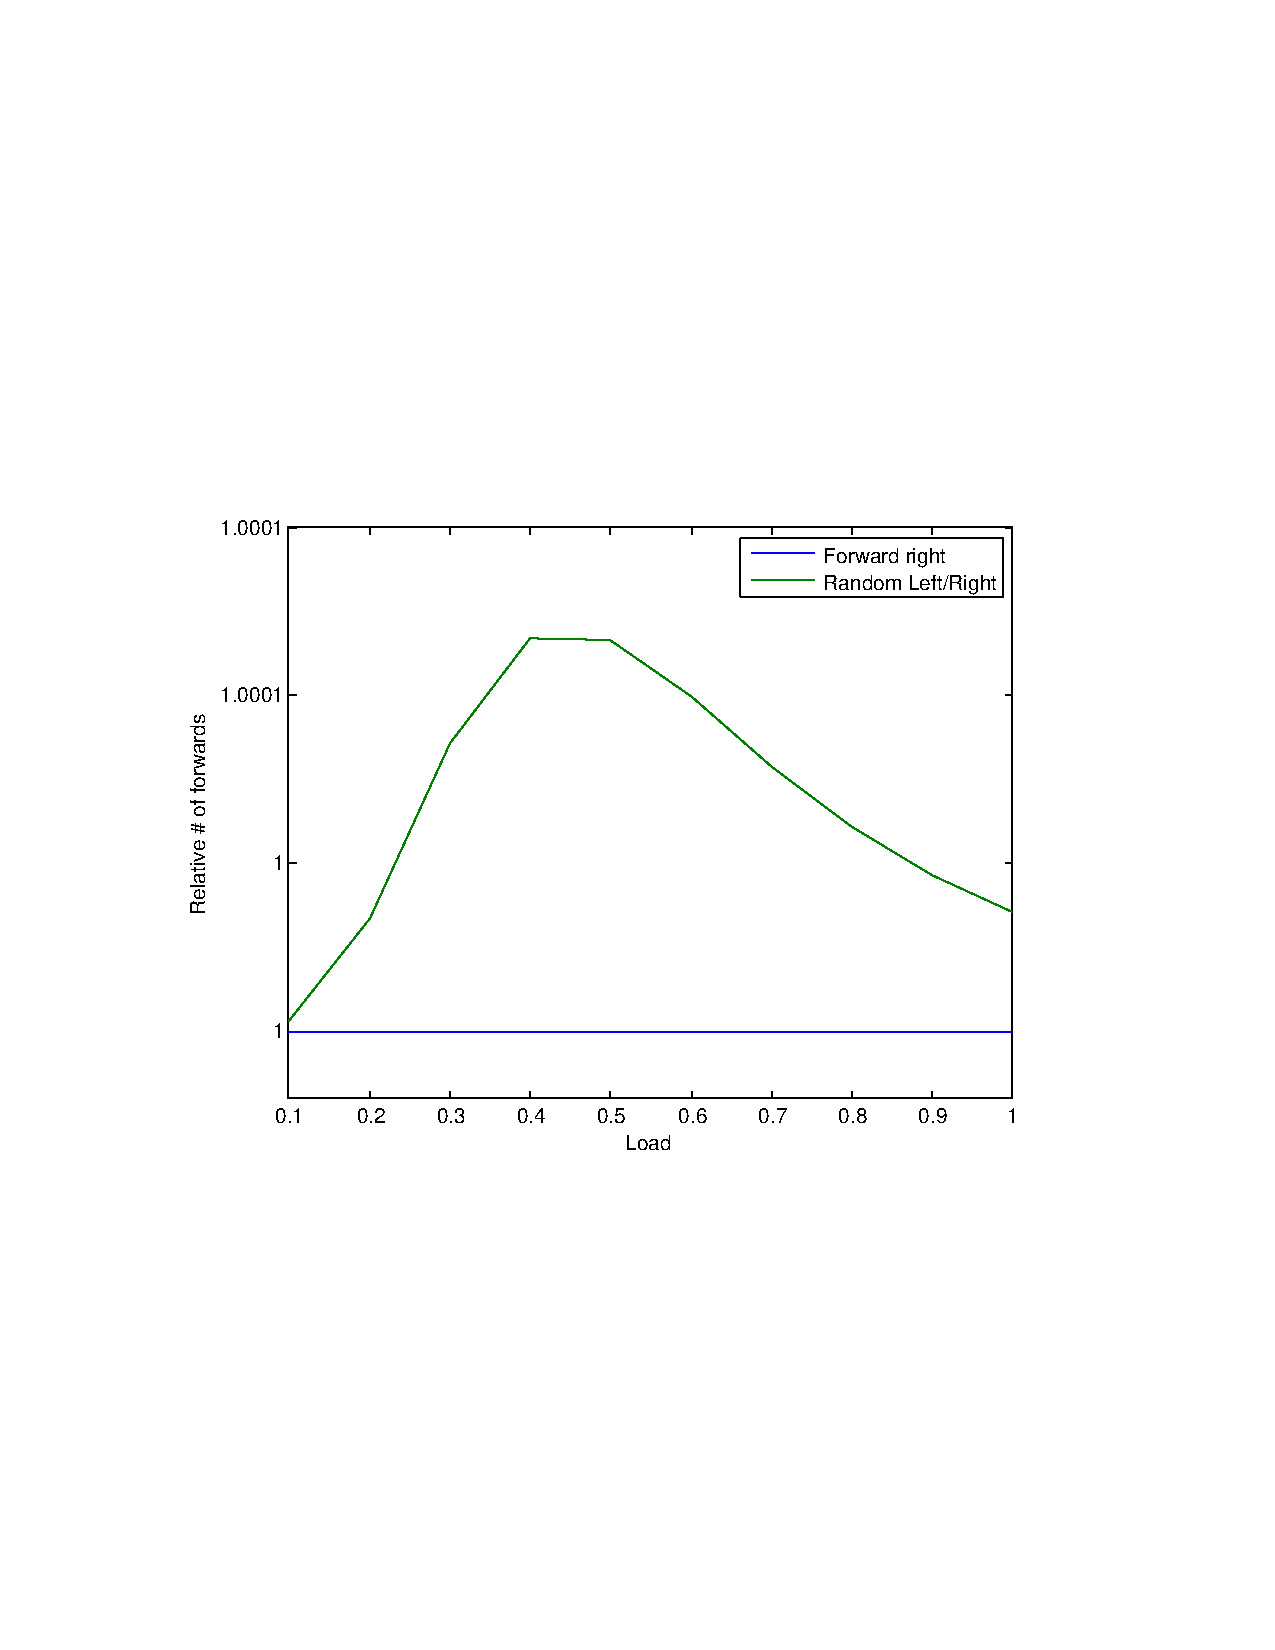
\includegraphics[clip=true, trim=9em 24em 9em 24em, width=0.9\textwidth]{resources/plotrandlr.pdf}
\caption{Validation of Random left/right with $p=0.5$}
\label{validrlr}
\end{figure}

It seems the results of the simulation fit. Although the results in \ref{validrlr} are much smoother than those in \ref{figrandswitch}, we must take into account that these results are computed exact and using a smaller ring size.

As in the simulation section, we have validated the results for different values of $p$. These results are shown in figure \ref{validrlrp}.

\begin{figure}[h!tb]
\centering
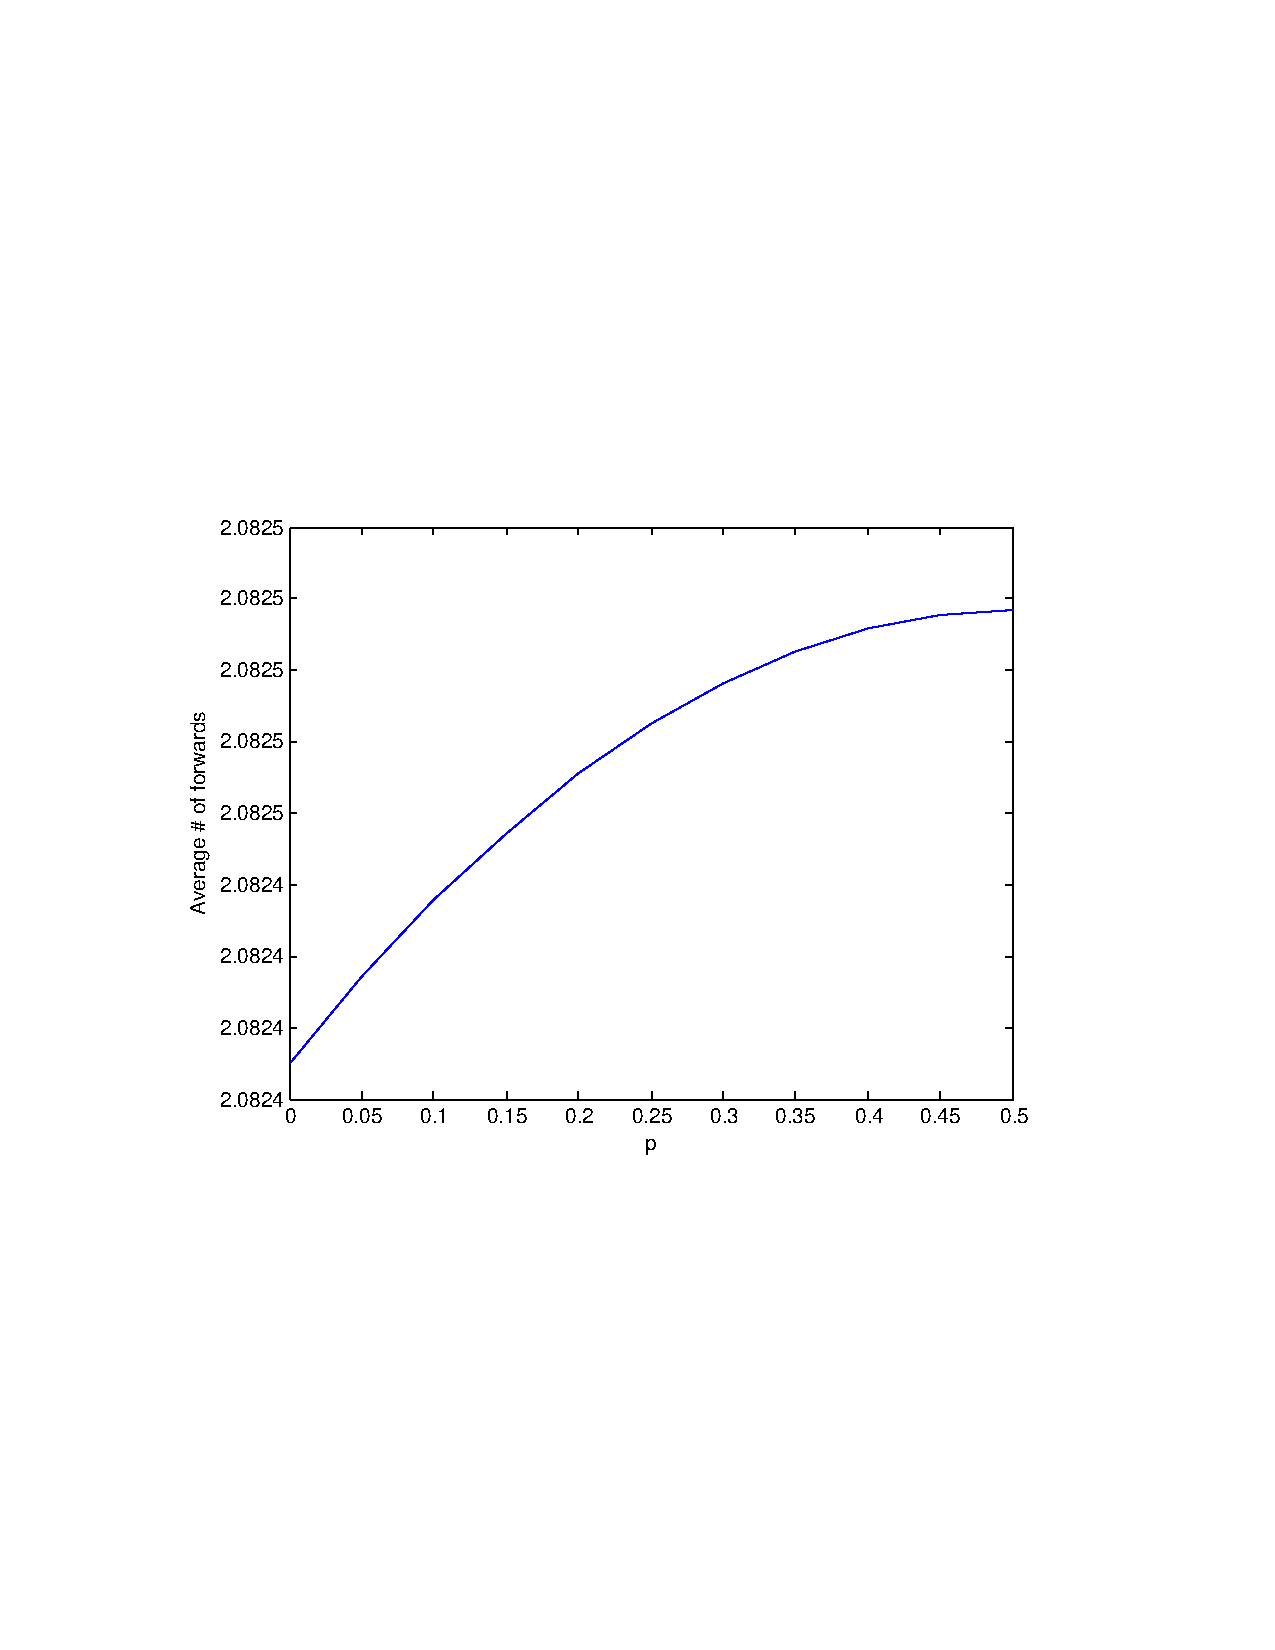
\includegraphics[clip=true, trim=9em 24em 9em 24em, width=0.9\textwidth]{resources/plotrandlrp.pdf}
\caption{Performance of random left/right with load$=0.8$}
\label{validrlrp}
\end{figure}

The random left/right forward algorithm does not seem a viable choice for real implementations. It has a small performance drawback compared to \FR and has no other benefits.

\subsubsection*{Random Unvisited}
This problem can be modeled much more efficiently than the techniques. Since the next node is chosen at random, it is not necessary to store the position of the nodes. The information we need to save consists only of the number of servers that are currently busy. This problem is similar to modeling an Erlang-B loss system. The number of states in this Markov Chain is linear to $N$, which is much more dense than the previous given models. For $N=3$, the matrix is given below.

\[ Q =
  \begin{blockarray}{ccccc}
    & 0 & 1 & 2 & 3 \\
    \begin{block}{c[cccc]}
    0 & -3\lambda & 3\lambda & 0 & 0 \\
    1 & \mu & -3\lambda-\mu & 3\lambda & 0 \\
    2 & 0 & \mu & -3\lambda-\mu & 3\lambda \\
    3 & 0 & 0 & \mu & -\mu \\
    \end{block}
  \end{blockarray}
\]

\subsubsection*{Random Coprime offset}
Modeling this technique yields different results for various ring sizes. The performance of this algorithm depends on $\varphi(N)$. The results in figure \ref{validcp} are very similar to those found in the simulation (figure \ref{figsimrcp}).

\begin{figure}
\centering
        \begin{subfigure}[b]{0.9\textwidth}
			\centering
			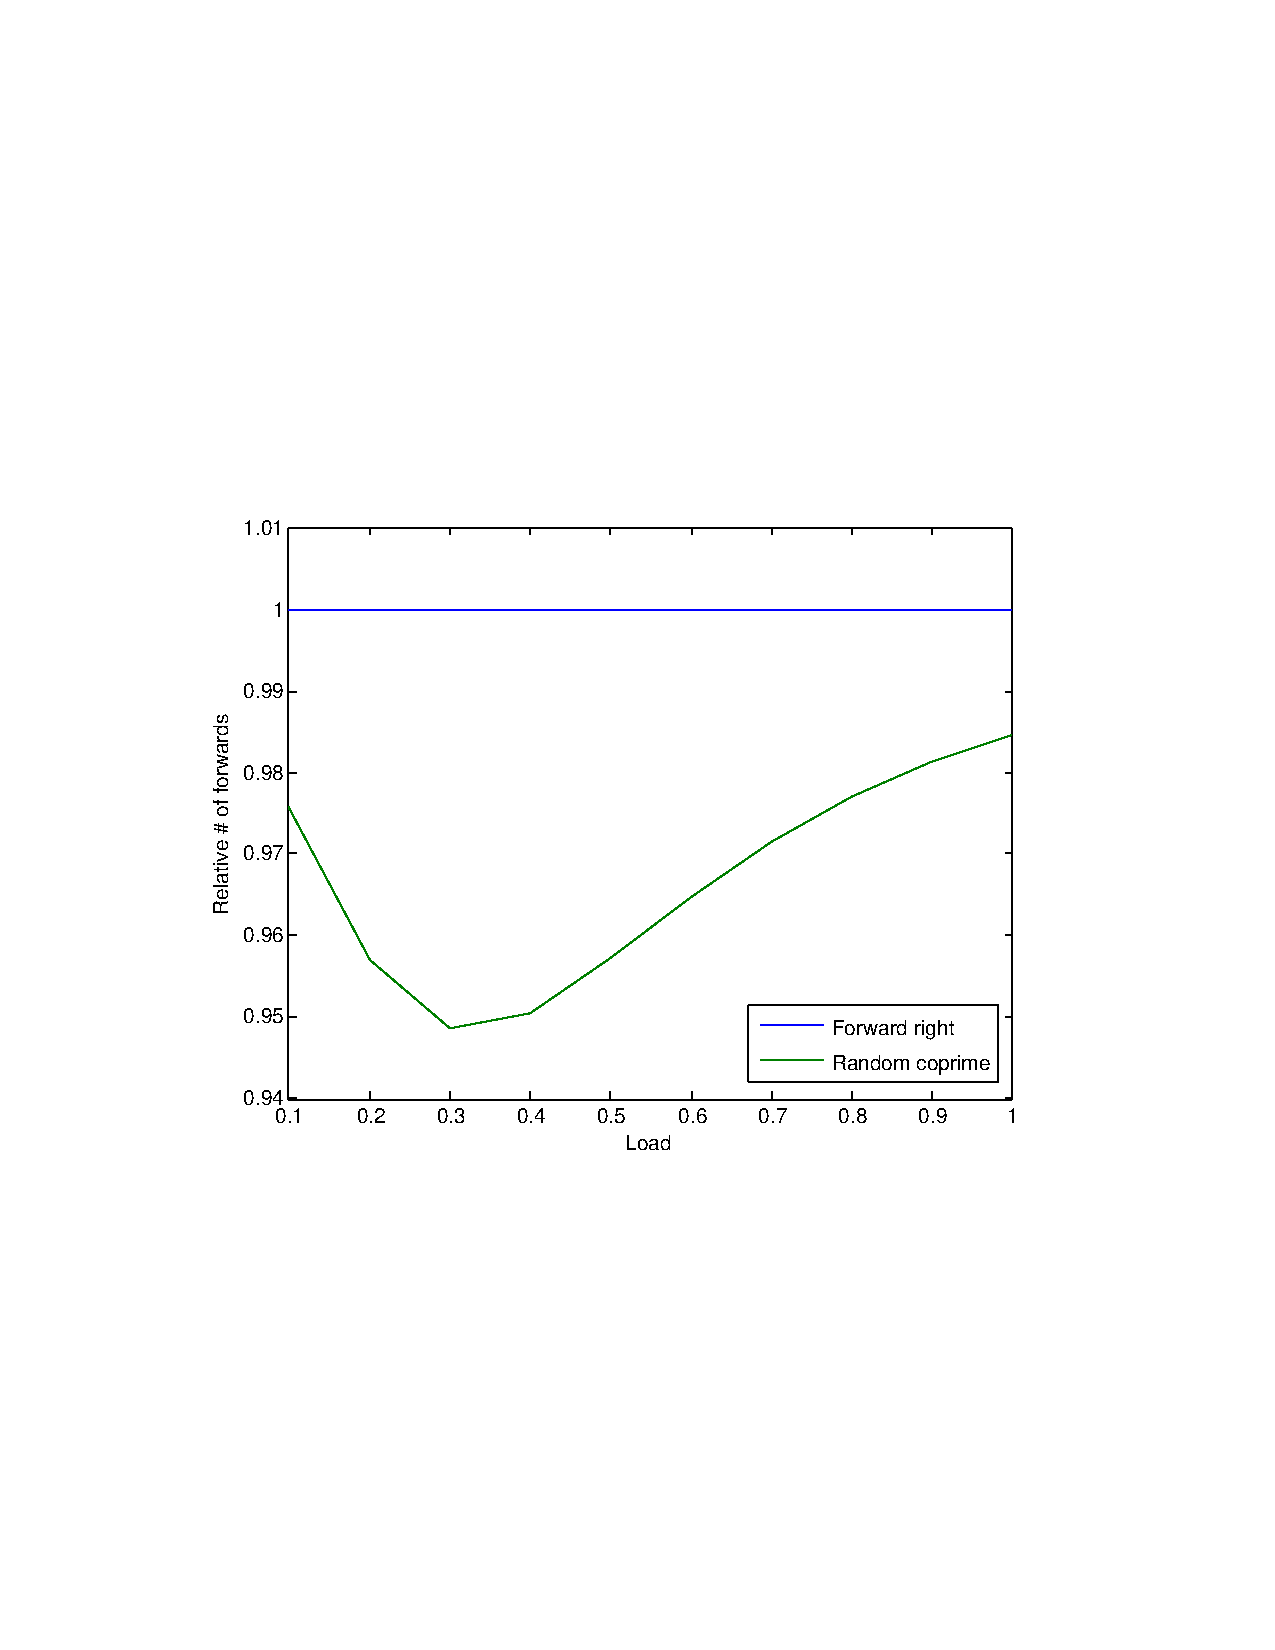
\includegraphics[clip=true, trim=9em 24em 9em 24em,width=\textwidth]{resources/plotrandcoprime.pdf}
			\caption{$N=10$}
			\label{validcp10}
        \end{subfigure}

		\begin{subfigure}[b]{0.49\textwidth}
			\centering
			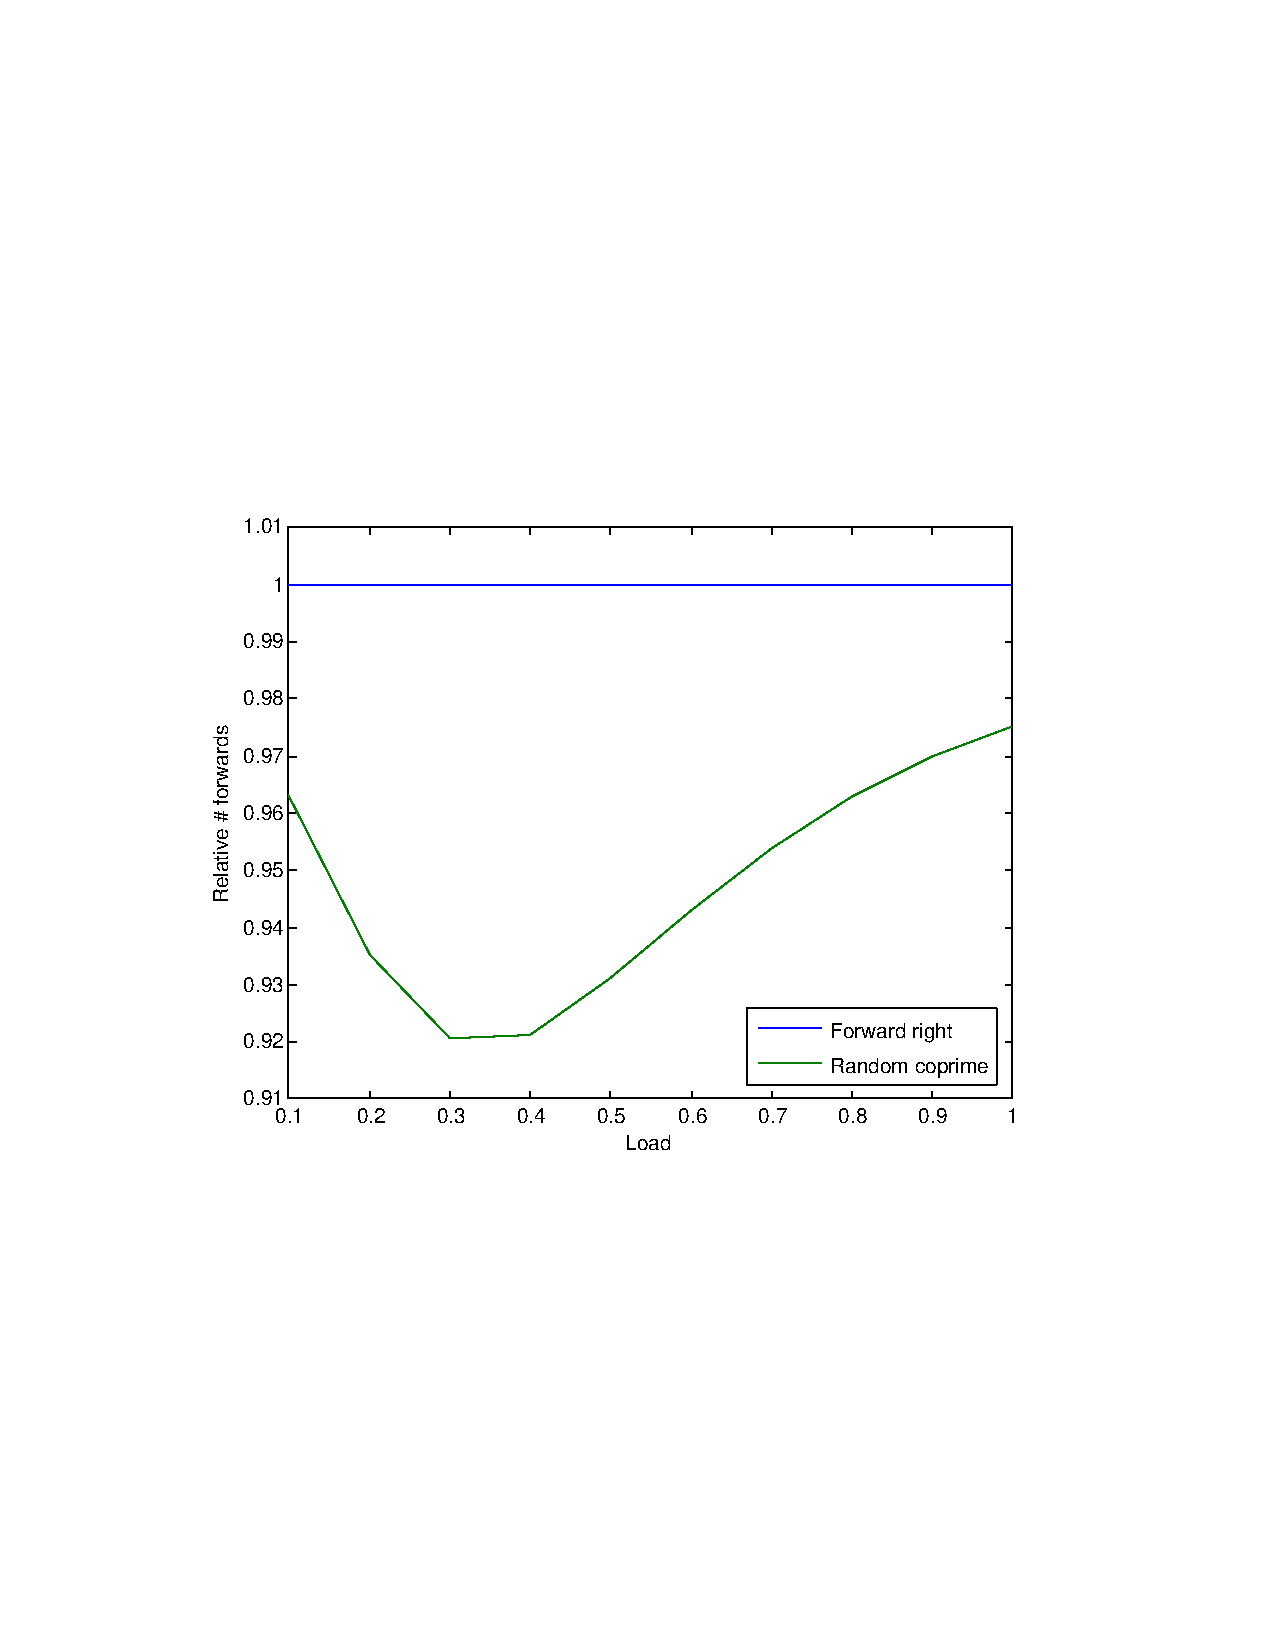
\includegraphics[clip=true, trim=9em 24em 9em 24em, width=\textwidth]{resources/plotrandcoprime11.pdf}
			\caption{$N=11$}
			\label{validcp11}
		\end{subfigure}
		\begin{subfigure}[b]{0.49\textwidth}
			\centering
			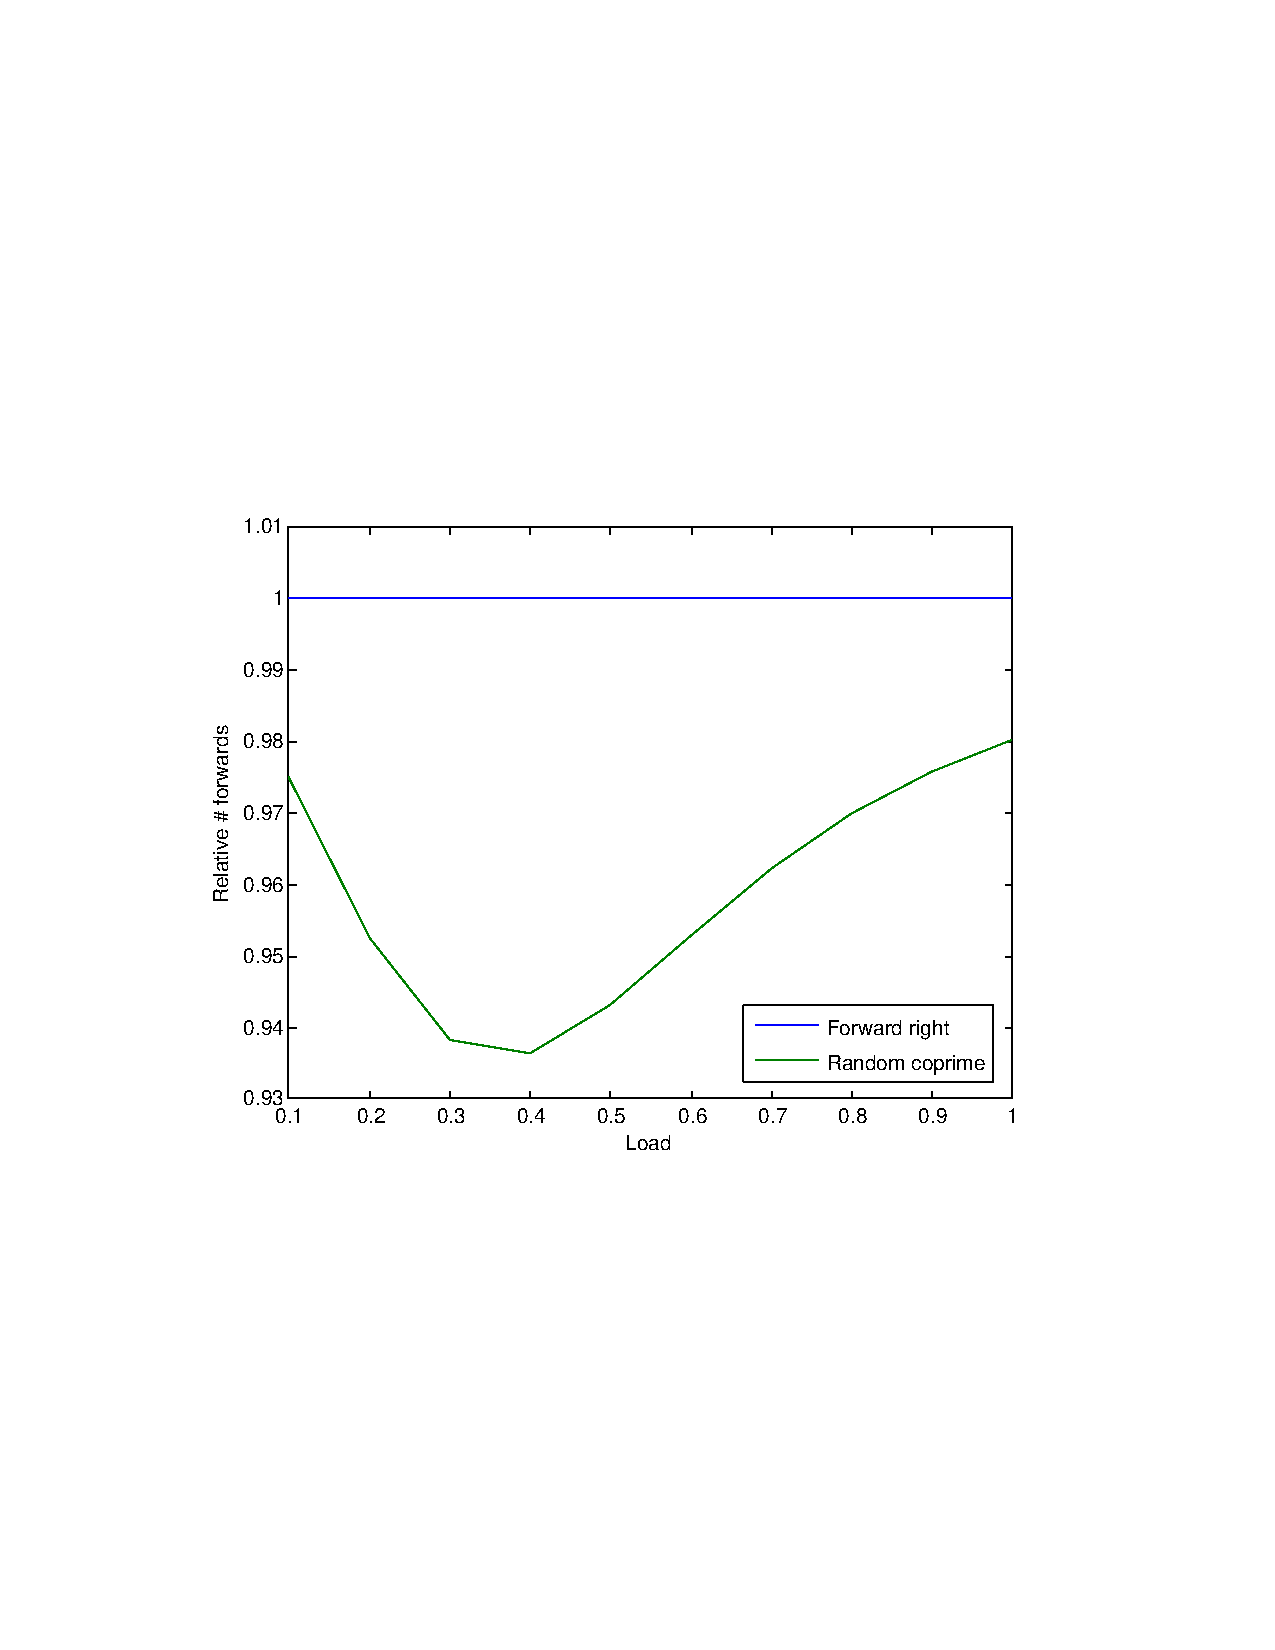
\includegraphics[clip=true, trim=9em 24em 9em 24em, width=\textwidth]{resources/plotrandcoprime12.pdf}
			\caption{$N=12$}
			\label{validcp12}
		\end{subfigure}
\caption{Validation of the Random Coprime offset algorithm}
\label{validcp}
\end{figure}

The results show a performance gain up to 5\% for a ring size of $N=10$. The list of coprimes in that scenario is ${1, 3, 7, 9}$, so 4 possible choices. When increasing the ring size to $11$, a prime number, the list of coprimes expands to ${1..10}$ (because 11 is prime), so 10 possible choices. This increases the relative performance gain up to 8\% (figure \ref{validcp11}). To make clear the increased performance is not due to the increase of $N$, figure \ref{validcp12} shows the performance gain for $N=12$. For $N=10$ and $N=12$, a job can follow 4 possible routes, for $N=11$, 10 different routes can be chosen.

\begin{figure}[h!tb]
\centering
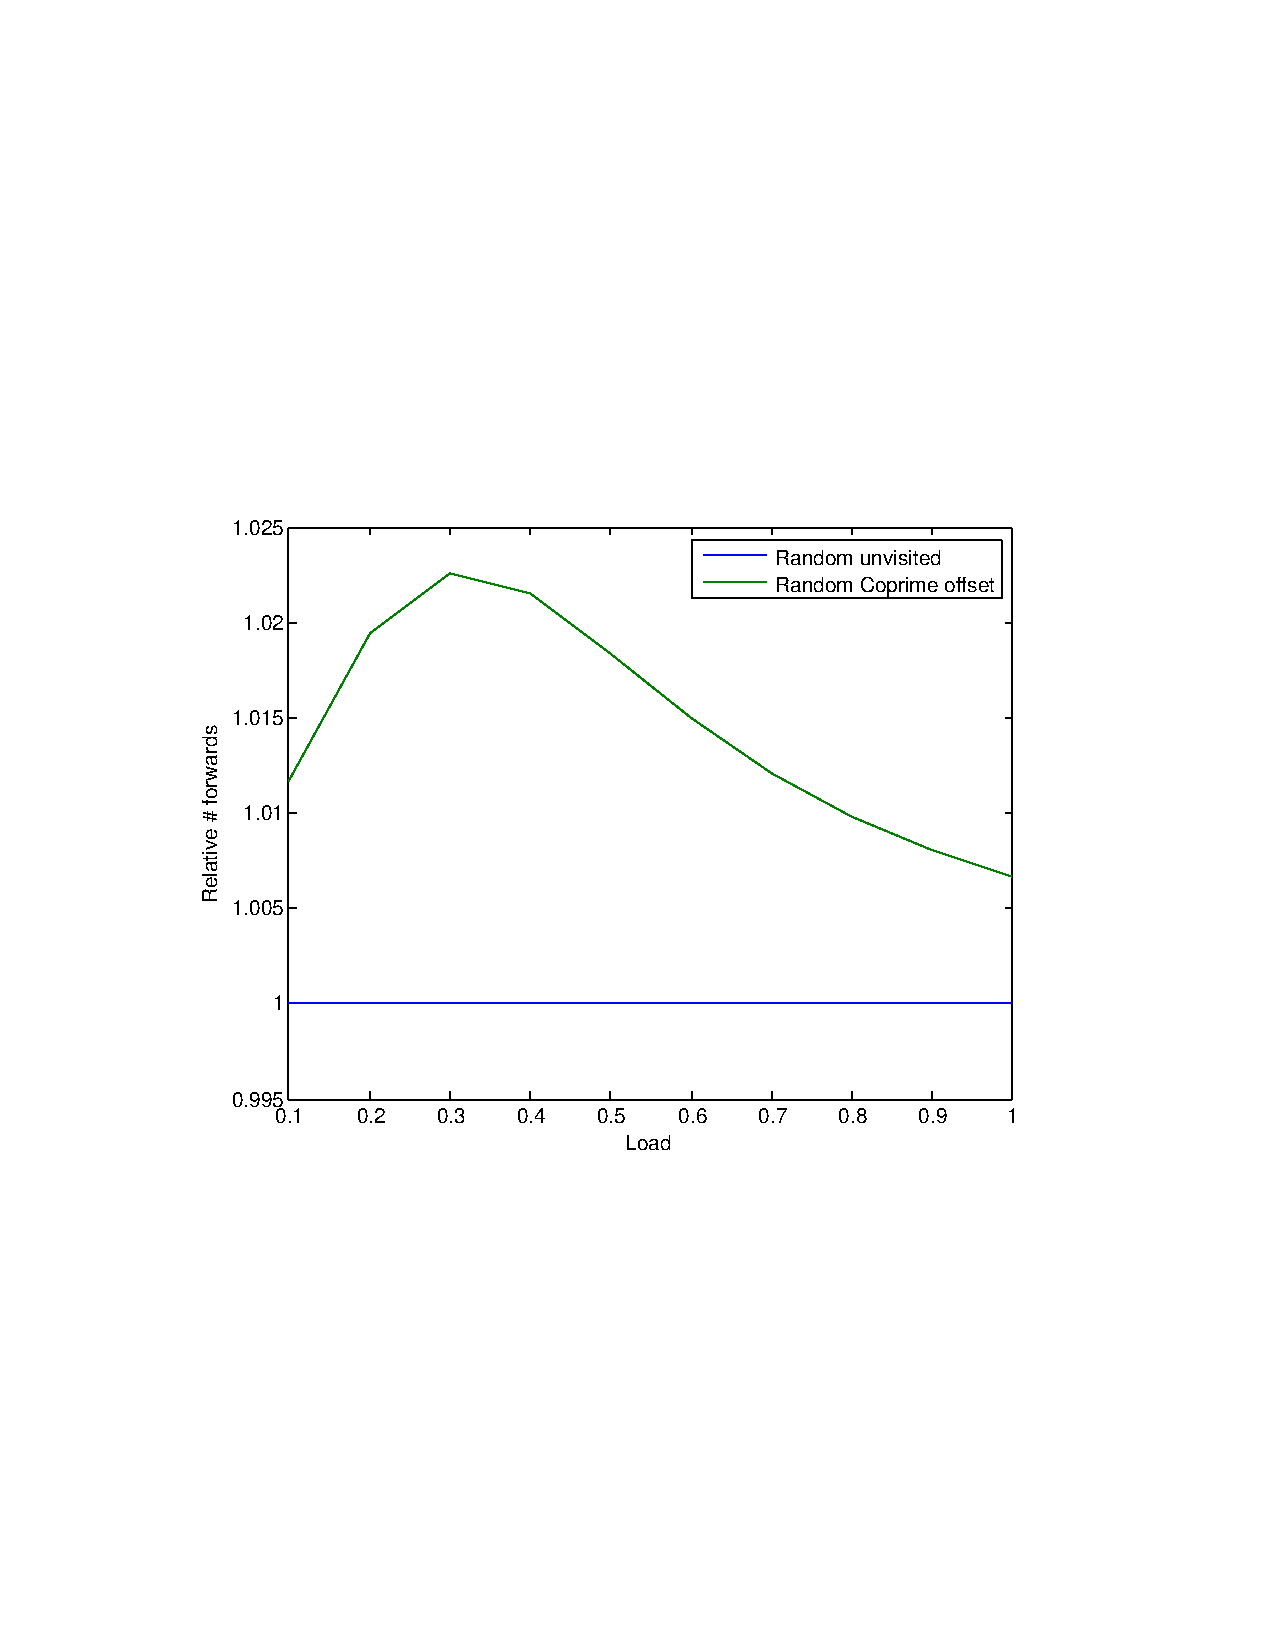
\includegraphics[clip=true, trim=9em 24em 9em 24em, width=0.9\textwidth]{resources/plotrandunvisitedrandprime.pdf}
\caption{Performance of Random Coprime offset relative to Random unvisited}
\label{figrurcpo}
\end{figure}

\subsection{Lumped states}
\label{lump}

Except for Random Unvisited, each described technique is modeled into a Markov Chain with $N^2$ states. However, many of these states are redundant: for example, for $N=3$ the states $001$, $010$ and $100$ all represent a state where one of the nodes is busy. For states representing multiple busy nodes, the space between these servers is critical information. Redundant states can be generated from one state: bitrotate the state by 1 until you get the original state. Each encountered state is redundant.
Example: the states below are redundant and can therefore be lumped into one state:
\begin{verbatim}
001101 = 011010 = 110100 = 101001 = 010011 = 100110
\end{verbatim}

The example model of the \FR algorithm can be lumped into the following Markov Chain:

\[ Q =
  \begin{blockarray}{ccccc}
    & 000 & 001 & 011 & 111 \\
    \begin{block}{c[cccc]}
    000 & -3\lambda & 3\lambda & 0 & 0 \\
    001 & \mu & 3\lambda-\mu & 3\lambda & 0 \\
    011 & 0 & 2\mu & 3\lambda-2\mu & 3\lambda \\
    111 & 0 & 0 & 3\mu & -3\mu \\
    \end{block}
  \end{blockarray}
\]

Computing the steady state distribution of a Markov Chain is subject to both time and memory constraints. Using sparse matrices for our algorithms reduces the memory constraint so much it is no longer a bottleneck.
Two factors are important when working with matrices: the number of elements and the number of nonzero elements. We will show that both factors are reduced significantly by lumping the matrices.

For unlumped Markov Chains modeling the Random forward algorithm, a matrix consists of $2^N$ states, an exponential growth. Lumping these matrices results in a number of states equal to  $\frac{1}{N} \sum_{d|N} (2^{N/d} \cdot \varphi(d) )$ \cite{A000031}. Although this result greatly reduces the number of states, its complexity is still non-polynomial.

The number of nonzero elements for unlumped Markov Chains is $(N+1) 2^N$. For lumped matrices, we were not able to derive an exact formula, however, figure \ref{lumpnnz} shows a clear reduction as well. Yet, this result does not seem polynomial either.

\begin{figure}[h!tb]
\centering
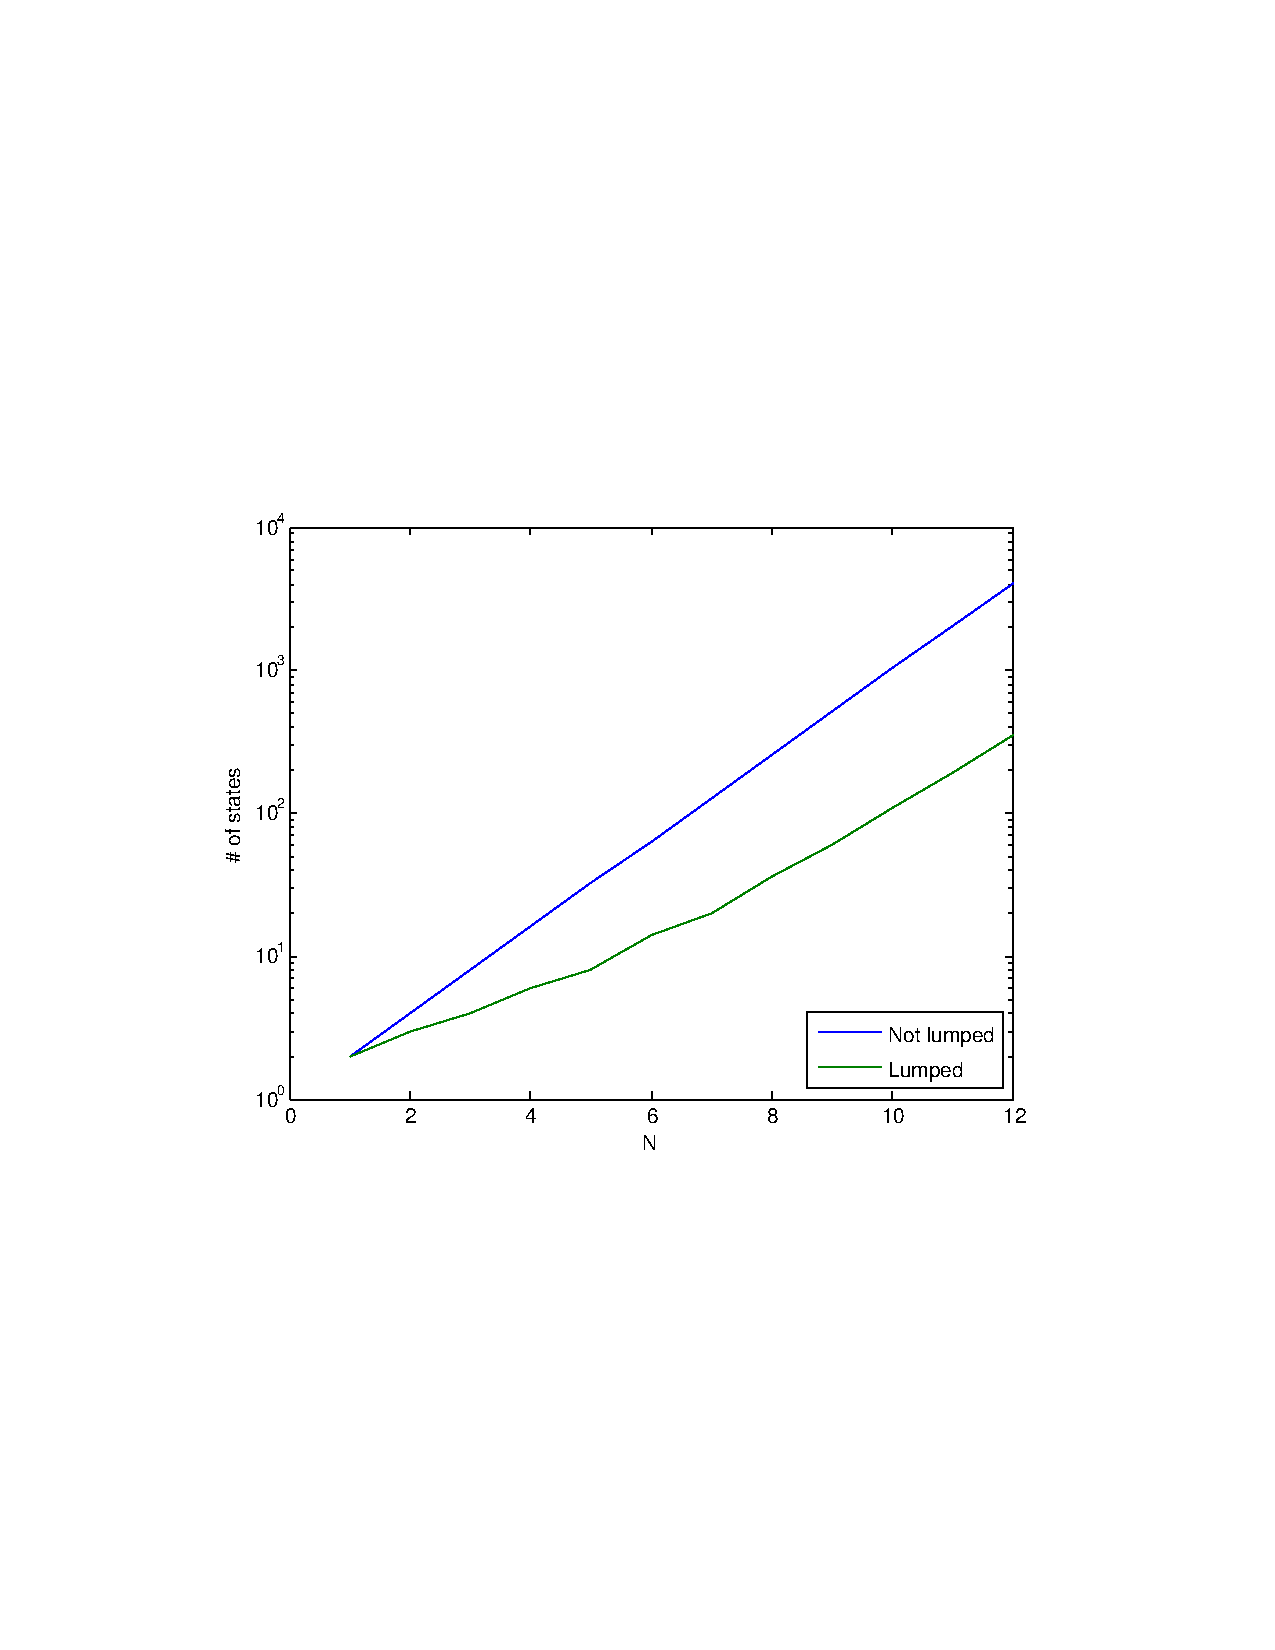
\includegraphics[clip=true, trim=9em 24em 9em 24em, width=0.9\textwidth]{resources/plotlumping.pdf}
\caption{Number of states}
\label{figlump}
\end{figure}

\begin{figure}[h!tb]
\centering
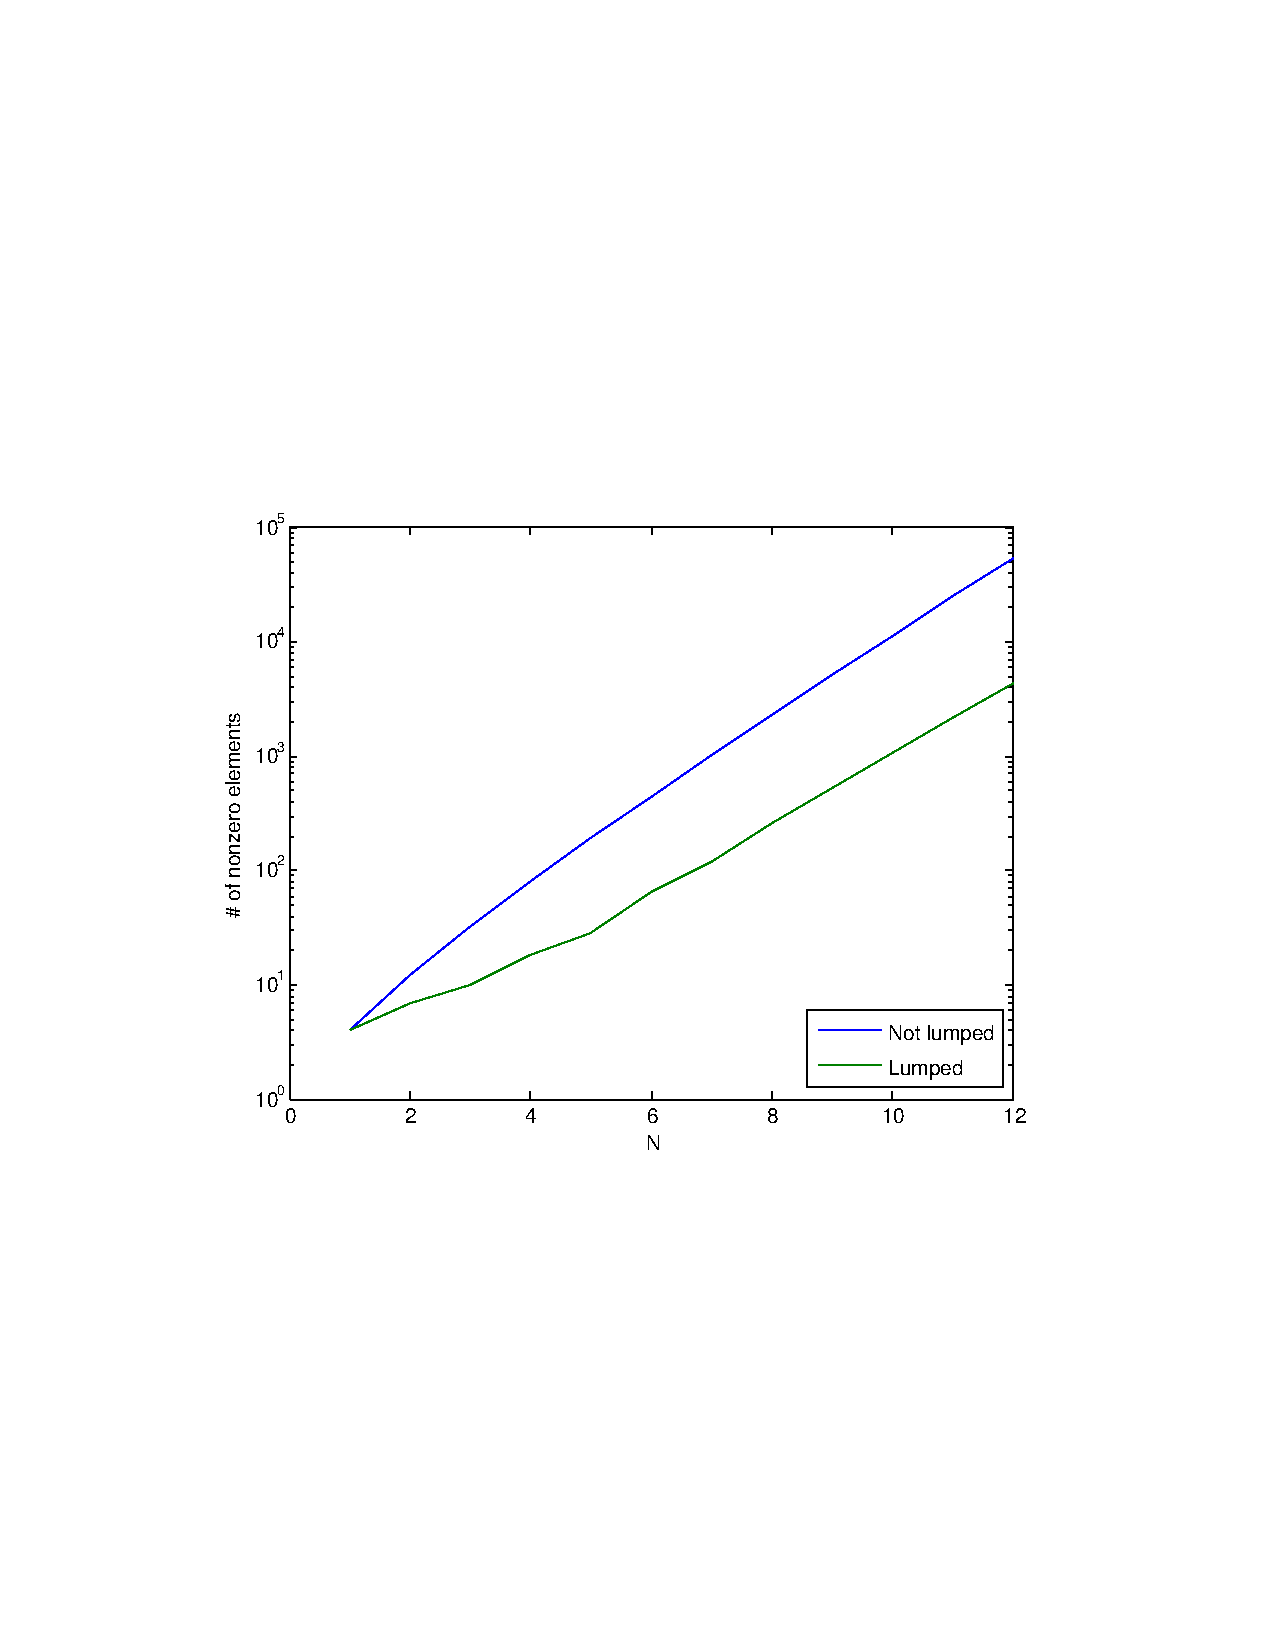
\includegraphics[clip=true, trim=9em 24em 9em 24em, width=0.9\textwidth]{resources/plotlumpingnnz.pdf}
\caption{Number of nonzero elements}
\label{lumpnnz}
\end{figure}

It seems lumping is a good technique to push the boundaries of the validation by reducing two important factors of the computing time. However, it is no silver bullet: both the number of states and the number of nonzero elements are non-polynomial after lumping the matrices.

\subsection{Equivalent algorithms}
Various algorithms are equivalent or very similar under special conditions. We will discuss some of these equivalencies.

\subsubsection*{Low N}
For $N \leq 3$ all algorithms are equivalent. This is obvious for $N=2$. For $N=3$, there are 4 possible states with the same behavior for each algorithm:
\begin{description}
\item[All nodes idle] All 3 nodes are idle, an incoming job will be executed by first node.
\item[1 node busy] Each node is as likely to be the next node receiving a job. For an idle node, the job is executed by that node. For the busy node, the job will need to make exactly 1 hop.
\item[2 node busy] Since each node is as likely to be the next node receiving a job, the job will be forwarded 0,1 or 2 times, all with the same probability.
\item[Saturated] The job will be dropped.
\end{description}

For $N>3$, other equivalencies exist. These are described below.

\subsubsection*{High load}
When the load becomes sufficiently large, all algorithms will yield the same results. In a ring under heavy load, each node will be busy nearly all the time. As long all nodes are busy, incoming jobs will be dropped.
When a node becomes idle, the first event will be an incoming job. The first incoming job will claim this node. Each node has the same probability of receiving the next incoming job, so the expected value for the number of forwards is:

\begin{eqnarray}
\frac{1}{N} \cdot \sum_{i=0}^{N-1} i &=& \frac{1}{N} \cdot \frac{N(N-1)}{2} \nonumber \\
&=& \frac{N-1}{2} \nonumber
\end{eqnarray}

\subsubsection*{Random left/right with parameter $p$ versus forward right}
This algorithm is always equivalent to itself using parameter $1-p$. This is intuitively clear because the probabilities of right and left are swapped, like looking to the ring in a mirror.
It is clear that for $p=0$ (and so for $p=1$), this algorithm is equivalent to the \FR algorithm. Furthermore, for arbitrary values of $p$, this algorithm is still equivalent to \FR as long as the ring size $N \leq 5$. This can be proven by lumping the Markov Chains for both techniques.

For $N=4$, define the lumped Markov Chain of the \FR algorithm.
\[ Q_1 =
  \begin{blockarray}{ccccccc}
    & 0000 & 0001 & 0011 & 0101 & 0111 & 1111 \\
    \begin{block}{c[cccccc]}
    0000 & -4\lambda & 4\lambda & 0 & 0 & 0 & 0 \\
    0001 & \mu & -4\lambda-\mu & 3\lambda & \lambda & 0 & 0 \\
    0011 & 0 & 2\mu & -4\lambda-2\mu & 0 & 4\lambda & 0 \\
    0101 & 0 & 2\mu & 0 & -4\lambda-2\mu & 4\lambda & 0  \\
    0111 & 0 & 0 & 2\mu & \mu & -4\lambda-3\mu & 4\lambda \\
    1111 & 0 & 0 & 0 & 0 & 4\mu & -4\mu \\
    \end{block}
  \end{blockarray}
\]

Now, define the lumped Markov Chain of the FR algorithm with parameter $p$ and simplify.

\[ Q_2 =
  \begin{blockarray}{ccccccc}
    & 0000 & 0001 & 0011 & 0101 & 0111 & 1111 \\
    \begin{block}{c[cccccc]}
    0000 & -4 \lambda & 4\lambda & 0 & 0 & 0 & 0 \\
    0001 & \mu & -\mu & \lambda + (1-p)\lambda+p\lambda+\lambda & \lambda & 0 & 0 \\
    0011 & 0 & 2\mu & -2\mu & 0 & \lambda+2\lambda \cdot ((1-p)+p)+\lambda & 0 \\
    0101 & 0 & 2\mu & 0 & -2\mu & \lambda+p\lambda+(1-p)\lambda & 0  \\
    0111 & 0 & 0 & 2\mu & \mu & -x & 4\lambda \\
    1111 & 0 & 0 & 0 & 0 & 4\mu & -4\mu \\
    \end{block}
  \end{blockarray}
\]
\[ Q_2 =
  \begin{blockarray}{ccccccc}
    & 0000 & 0001 & 0011 & 0101 & 0111 & 1111 \\
    \begin{block}{c[cccccc]}
    0000 & -4\lambda & 4\lambda & 0 & 0 & 0 & 0 \\
    0001 & \mu & -4\lambda-\mu & 3\lambda & \lambda & 0 & 0 \\
    0011 & 0 & 2\mu & -4\lambda-2\mu & 0 & 4\lambda & 0 \\
    0101 & 0 & 2\mu & 0 & -4\lambda-2\mu & 4\lambda & 0  \\
    0111 & 0 & 0 & 2\mu & \mu & -4\lambda-3\mu & 4\lambda \\
    1111 & 0 & 0 & 0 & 0 & 4\mu & -4\mu \\
    \end{block}
  \end{blockarray}
\]

We find $Q_1 = Q_2$ for $N=4$. This also works for $N=5$, but for $N \geq 6$, the matrices are different.

\subsubsection*{Random Coprime offset versus forward right}
For $N=4$, this algorithm is equivalent to the \FR algorithm as well. The coprimes of 4 are 1 and 3. Meaning a jump of 1 (right neighbor) or a jump of 3 (left neighbor). It is clear this is the same as \RLRF{0.5}, which is equivalent to the \FR algorithm.

\subsubsection*{Random Coprime offset versus Random unvisited}
The performance of the Random Coprime offset algorithm depends on $\varphi(N)$, which is $N-1$ when $N$ is prime. Figure \ref{figrcovsru} shows the average ring traversal of this algorithm and the Random unvisited algorithm. It seems for prime values of $N$, the graphs touch. However, when looking at the actual data we see this is only true for $N=5$.

\begin{figure}[h!tb]
\centering
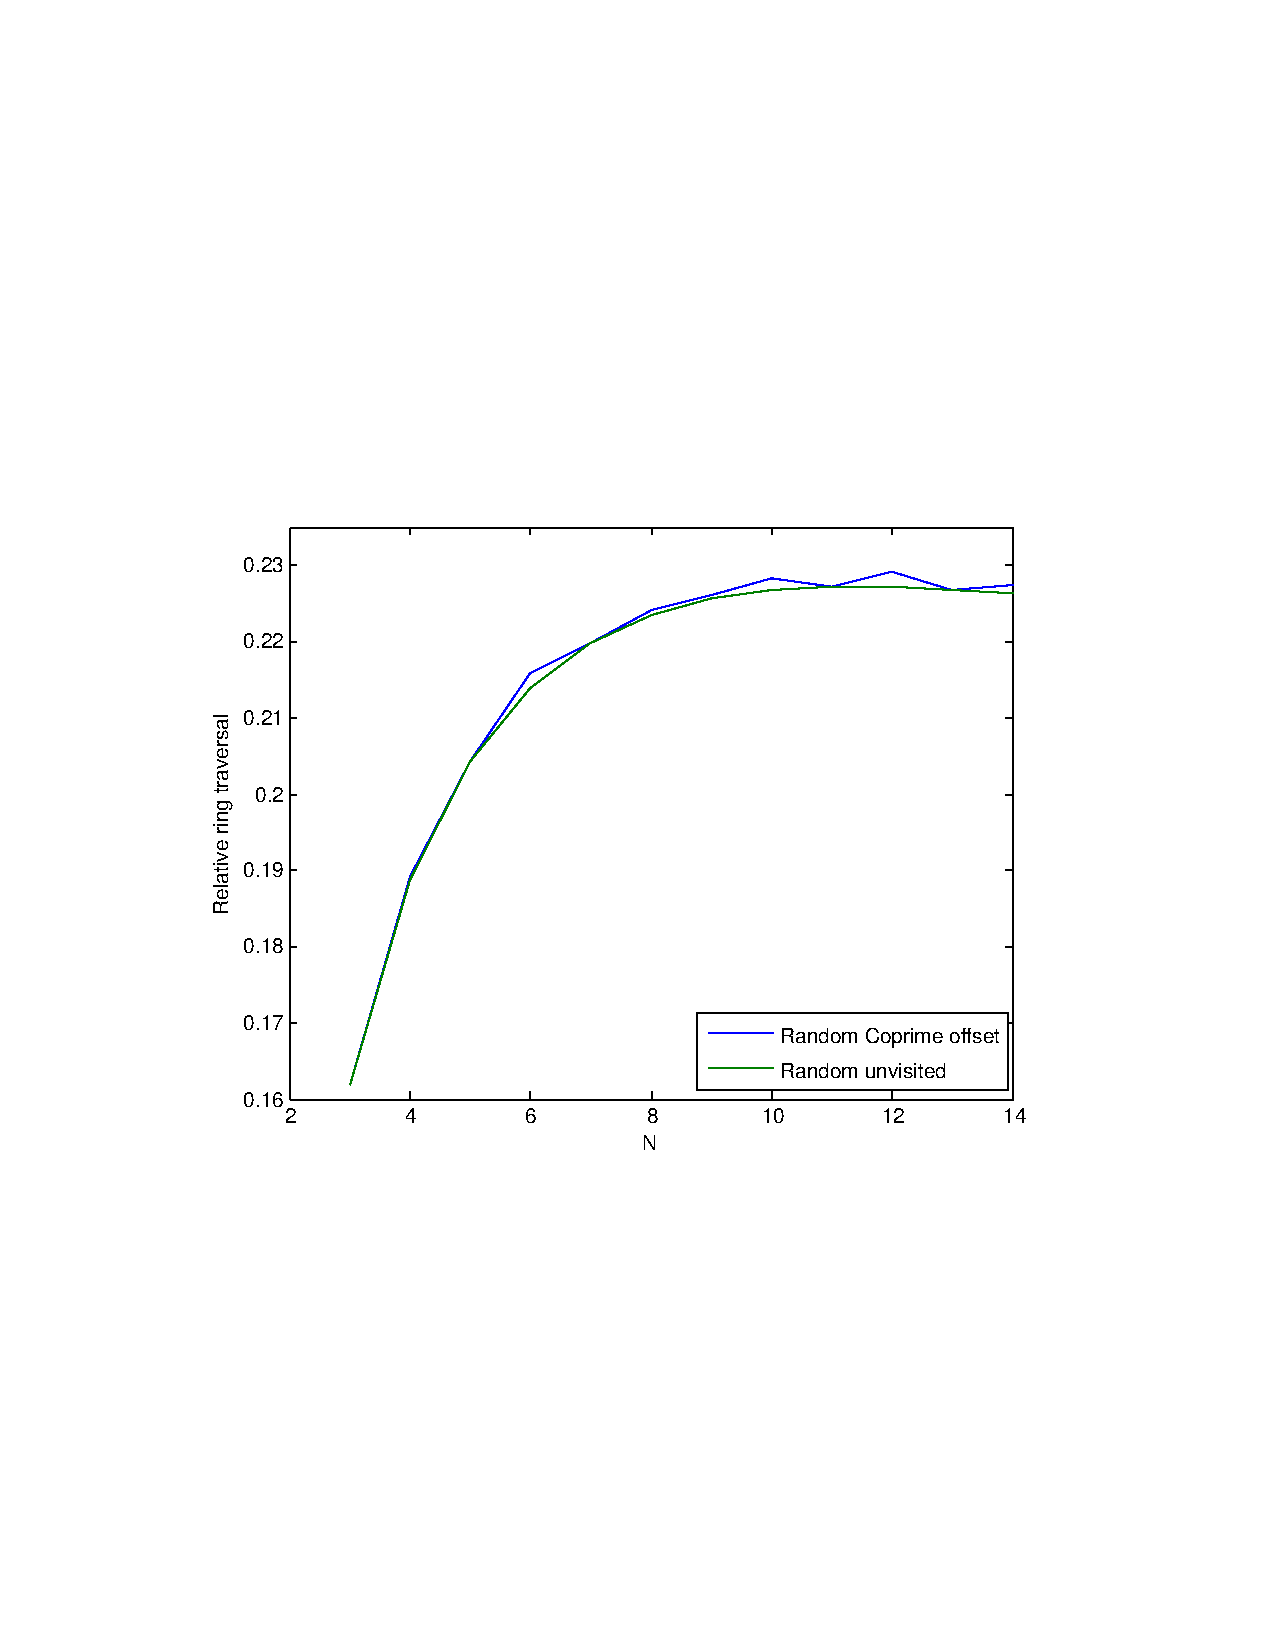
\includegraphics[clip=true, trim=9em 24em 9em 24em, width=0.9\textwidth]{resources/plotload10rurpo.pdf}
\caption{Ring traversal versus $N$ for load=1.0}
\label{figrcovsru}
\end{figure}

\begin{table}[h!]
\centering
\begin{tabular}{|l|l|l|} \hline
N	& Random unvisited	& Random Coprime offset \\ \hline
3	&   0.161764705882353 &  0.161764705882353 \\
5	&   0.204376460590610 &  0.204376460590610 \\
7	&   0.219792926622134 &  0.219788935482327 \\
11	&   0.227265522566042 &  0.227249844727623 \\
13	&   0.226908433098761 &  0.226887197455899 \\ \hline
\end{tabular}
\caption{Relative ring traversal for load=1.0}
\end{table}

\section{Conclusion}
\label{secconclusion}

We have simulated all our algorithms and validated the results of some of them. The ideal algorithm is depends on the specific requirements of the distributed system. However, it is safe to say some algorithms are not ideal for any situation. One should also note that in some configurations, different algorithms can yield the same results. In those cases, only memory requirements or the complexity to implement the algorithms should be decisive.

\subsubsection*{Forward to neighbors}
When nodes are only directly connected to their neighbors, the choice depend on the memory requirements. When at least 1 bit can be saved in both the job's metadata as the node's state, \LRF is an ideal choice. This algorithm provides up to 4\% better result than \FR under medium load ($N=100$).

When no memory is available, the \FR algorithm is the only possible choice while maintaining sufficient results. Additionally, it is the easiest algorithm to implement.

Both these algorithms allow nodes to come and go. The random left/right and Position dependent forwarding techniques perform worse than \FR while having more requirements, therefore they should not be chosen.

\subsubsection*{Forward anywhere}
If each node can reach each other node directly, the forward anywhere algorithms improve the results significantly. The best results can be achieved using the Random unvisited algorithm. This algorithm performs slightly better than coprime offset and random Coprime offset, but at a higher cost: the random unvisited algorithm requires $N-1$ bits in the job's metadata.

The Coprime offset and Random Coprime offset algorithms require less memory but with worse performance. However, when the ring size is prime, its results are only slightly less than those of random unvisited. The memory required in the job's metadata is lowered to $\lceil log_2 \varphi(N) \rceil$ bits ($\lceil log_2 (N-1) \rceil$ bits when $N$ is prime). The coprime offset algorithm yields about the same results as the random variant. In addition, it needs to save $\lceil log_2 \varphi(N) \rceil$ bits in the state of each node. Random coprime offset and random unvisited seem two very good candidates, it depends whether the small performance benefit is worth the memory and implementation cost.

\subsubsection*{Other findings}
The results of using multiple CPUs per server can be approximated using the the results of 1 CPU per server and a ring size $N_1 = N_c \cdot c$. This approximation is an upper bound to the real outcome since the derivation ignores the fact that the choice for a node is no longer a choice for a CPU, it is a choice for a group of $c$ CPUs. 

For the \RLRF{$p$}, we have found out its results are worst for $p=0.5$. We did not come up with an explanation why this algorithm is worse than \FR. This might be a start for further research.

We have also found a way to model some of these algorithms into Markov Chains. This allowed us to compute the actual result of a simulation. The drawback of our model is the limited ring size. We optimized it by lumping states and using sparse matrices, but because of the non-polynomial nature of the matrix size, these optimizations allow us to increase $N$ only by 2 or 3.

Another finding is the equivalency between multiple algorithms, under certain conditions some algorithms model the exact same problem.

\printbibliography
\begin{changemargin}{-2cm}{-2cm}{4cm}
\newpage
\appendix
\section{Simulator source code}
\label{sourcecode}


\lstset{tabsize=4,language=C++,caption={Main.cpp}}
\lstinputlisting{../src/Main.cpp}

\lstset{caption={configuration.h}}
\lstinputlisting{../src/configuration.h}

\lstset{caption={configuration.cpp}}
\lstinputlisting{../src/configuration.cpp}

\lstset{caption={nodes.h}}
\lstinputlisting{../src/nodes.h}

\lstset{caption={nodes.cpp}}
\lstinputlisting{../src/nodes.cpp}

\lstset{caption={servernode.h}}
\lstinputlisting{../src/servernode.h}

\lstset{caption={servernode.cpp}}
\lstinputlisting{../src/servernode.cpp}

\lstset{caption={ring/arriveevent.h}}
\lstinputlisting{../src/ring/arriveevent.h}

\lstset{caption={ring/finishevent.h}}
\lstinputlisting{../src/ring/finishevent.h}

\lstset{caption={ring/job.h}}
\lstinputlisting{../src/ring/job.h}

\lstset{caption={ring/job.cpp}}
\lstinputlisting{../src/ring/job.cpp}

\lstset{caption={ring/node.h}}
\lstinputlisting{../src/ring/node.h}

\lstset{caption={ring/node.cpp}}
\lstinputlisting{../src/ring/node.cpp}

\lstset{caption={ring/ring.h}}
\lstinputlisting{../src/ring/ring.h}

\lstset{caption={ring/ring.cpp}}
\lstinputlisting{../src/ring/ring.cpp}

\lstset{caption={simulator/event.h}}
\lstinputlisting{../src/simulator/event.h}

\lstset{caption={simulator/schedule.h}}
\lstinputlisting{../src/simulator/schedule.h}

\lstset{caption={simulator/schedule.cpp}}
\lstinputlisting{../src/simulator/schedule.cpp}

\lstset{caption={simulator/simulator.h}}
\lstinputlisting{../src/simulator/simulator.h}

\lstset{caption={simulator/simulator.cpp}}
\lstinputlisting{../src/simulator/simulator.cpp}

\newpage
\section{MATLAB Numerical evaluation code}
\label{matlabcode}

\lstset{tabsize=8,language=Octave,caption={rightchain.m}}
\lstinputlisting{../matlab/rightchain.m}

\lstset{caption={randswitchchain.m}}
\lstinputlisting{../matlab/randswitchchain.m}

\lstset{caption={rprimechain.m}}
\lstinputlisting{../matlab/rprimechain.m}

\lstset{caption={runvisitedchain.m}}
\lstinputlisting{../matlab/runvisitedchain.m}

\lstset{caption={avghops.m}}
\lstinputlisting{../matlab/avghops.m}

\lstset{caption={ruavghops.m}}
\lstinputlisting{../matlab/ruavghops.m}

\lstset{caption={ctmcsteadystate.m}}
\lstinputlisting{../matlab/ctmcsteadystate.m}

\lstset{caption={lumpavghops.m}}
\lstinputlisting{../matlab/lumpavghops.m}

\lstset{caption={lump.m}}
\lstinputlisting{../matlab/lump.m}

\lstset{caption={makestates.m}}
\lstinputlisting{../matlab/makestates.m}

\end{changemargin}

\end{document}